\documentclass{vivid_layout}

% \makeprint is for printing and trimming on paper, w/crop marks.
% \makeprint

%\usepackage{tikz}
%\usetikzlibrary{datavisualization}
%\usetikzlibrary{datavisualization.formats.functions}

%% Required to build cover page
\title{Everything You Need To Know About}{Scalability - DRAFT}
\date{\today{} \textbullet{} DRAFT \textbullet{} CORRECTIONS APPRECIATED}
\cover{scalability/cover}

%% Required to build "Meet the Author"
\author{Baron Schwartz}{img/baron}

%% Required image for "About VividCortex"
\aboutvc{img/presenter}

%% Required resource info
\resourceleft%
	{Everything You Need To Know About Queueing Theory}
	{This highly accessible
	introduction demystifies queueing theory without using pages full of equations,
	helping you build intuition about it.}
	{img/queueing-theory}
	{https://www.vividcortex.com/resources/queueing-theory/}
\resourceright%
	{Case Study: SendGrid}
	{VividCortex is the go-to solution
	for seeing what's happening in SendGrid's production systems. It has saved
	months of effort and made query performance data available instantly to the
	entire team.}
	{img/sendgrid-thumbnail}
	{https://www.vividcortex.com/resources/case-studies/sendgrid/}

\begin{document}
\maketitle		% Build the cover page
\begin{bio}		% Biographical info for "Meet the Author"
Baron is a performance and scalability expert who participates in various
database, opensource, and distributed systems communities. He has helped build
and scale many large, high-traffic services for Fortune 1000 clients. He has
written several books, including O'Reilly's best-selling High Performance MySQL.
Baron has a CS degree from the University of Virginia.
\end{bio}
\tableofcontents	% Build the table of contents

\section{Introduction}

Making systems big, fast, and efficient is one of the most interesting and
satisfying things I've done. It's a great feeling when you fix a bottleneck, and
get dramatically improved performance at scale. You suddenly realize how
wasteful your systems were before the improvement.

I've participated in lots of projects that have produced those kinds of outcomes.
It's no coincidence that the best results came from the projects where the most
disciplined analysis was performed up front. Like performance optimization,
scalability optimization can be a real mystery unless you have an accurate model
of how the world works, good measurements of how your systems are performing,
and the ability to identify the problem and its likely fix with high certainty.

What's even better than fixing problems with scalability is the ability to
design systems (and organizations) that scale in the first place. This is worth
its weight in gold.

Scalability is quite a scientific topic, but it doesn't need to be mysterious.
It's true that queueing theory is intimately involved, and queueing is
complicated and unintuitive. But what's really cool is that scalability,
correctly understood, is quite straightforward despite the complexity of what's
going on behind the scenes.

I wrote this book to help you understand the simple, but profoundly
powerful, truths about scalability. I also wanted to help you understand the
connections between scalability and other disciplines, such as performance
optimization or the study of queueing. My hope is that this book is as
transformational and rewarding for you as the process of learning these concepts
has been for me.

\newpage

\section{What is Scalability?}

Scalability is ambiguous for many people---a vague term often tossed about in
conference presentations, for example. It's often used in ways confusingly
similar to performance, efficiency, capacity, availability, and many other terms
related to making things big and fast.

Wikipedia's definition of scalability, borrowed from a 2000 paper by Andr\'e B.
Bondi, is ``the capability of a system, network, or process to
handle a growing amount of work, or its potential to be enlarged in order to
accommodate that growth.'' This isn't wrong, but it's still a bit informal, and
this book needs a more formal definition.

Dr. Neil J. Gunther provides one such definition: scalability is a {\itshape
function}. I read his books and heard him speak, but it was still a year or so
before I understood. {\itshape Scalability can be defined as a
mathematical function}, a relationship between independent and dependent
variables (input and output). This is the type of formal definition you need to
model and analyze scalability.

The most important part of understanding such a scalability model is choosing
the correct variables to describe the way systems really operate.  Bondi's
definition provides a good clue: {\itshape work} is the driving factor of
scalability. Useful ways to think about work include, to mention a few,

\begin{itemize}
\item Units of work (requests).
\item The rate of requests over time (arrival rate).
\item The number of units of work in a system at a time (concurrency).
\item The number of customers or users sending requests.
\end{itemize}

Each of these can play sensible roles in the scalability function, depending on
how you view it. For example, it's quite common to configure the number of
threads a benchmark runs to send requests to a database. The benchmark usually
sends requests as fast as possible, assuming zero think time, so the arrival
rate is related to, but not strictly controlled by,\footnote{Because it is
determined by how quickly the database finishes each request.} the benchmark
configuration.

You could say that the amount of work requested is the input to the benchmark's
scalability function, and the completion rate is the output.

In another scenario, you might vary the number of CPUs for the system under test
(SUT) while holding constant the load per CPU, or if it's a clustered database,
vary the cluster size and hold constant the load per node. In this case, the
independent variable is the system size and the dependent variable is the
completion rate.

In most cases I've analyzed, either size or load are the sensible
independent variables for the scalability function. So for the purposes of this
book, I'll consider scalability to be {\itshape a function of size or load}.
The dependent variable will be the rate at which the system can complete work,
or {\itshape throughput}. The hope is that the system should complete more work
as size or load grow, so it should be an increasing function.
\begin{center}
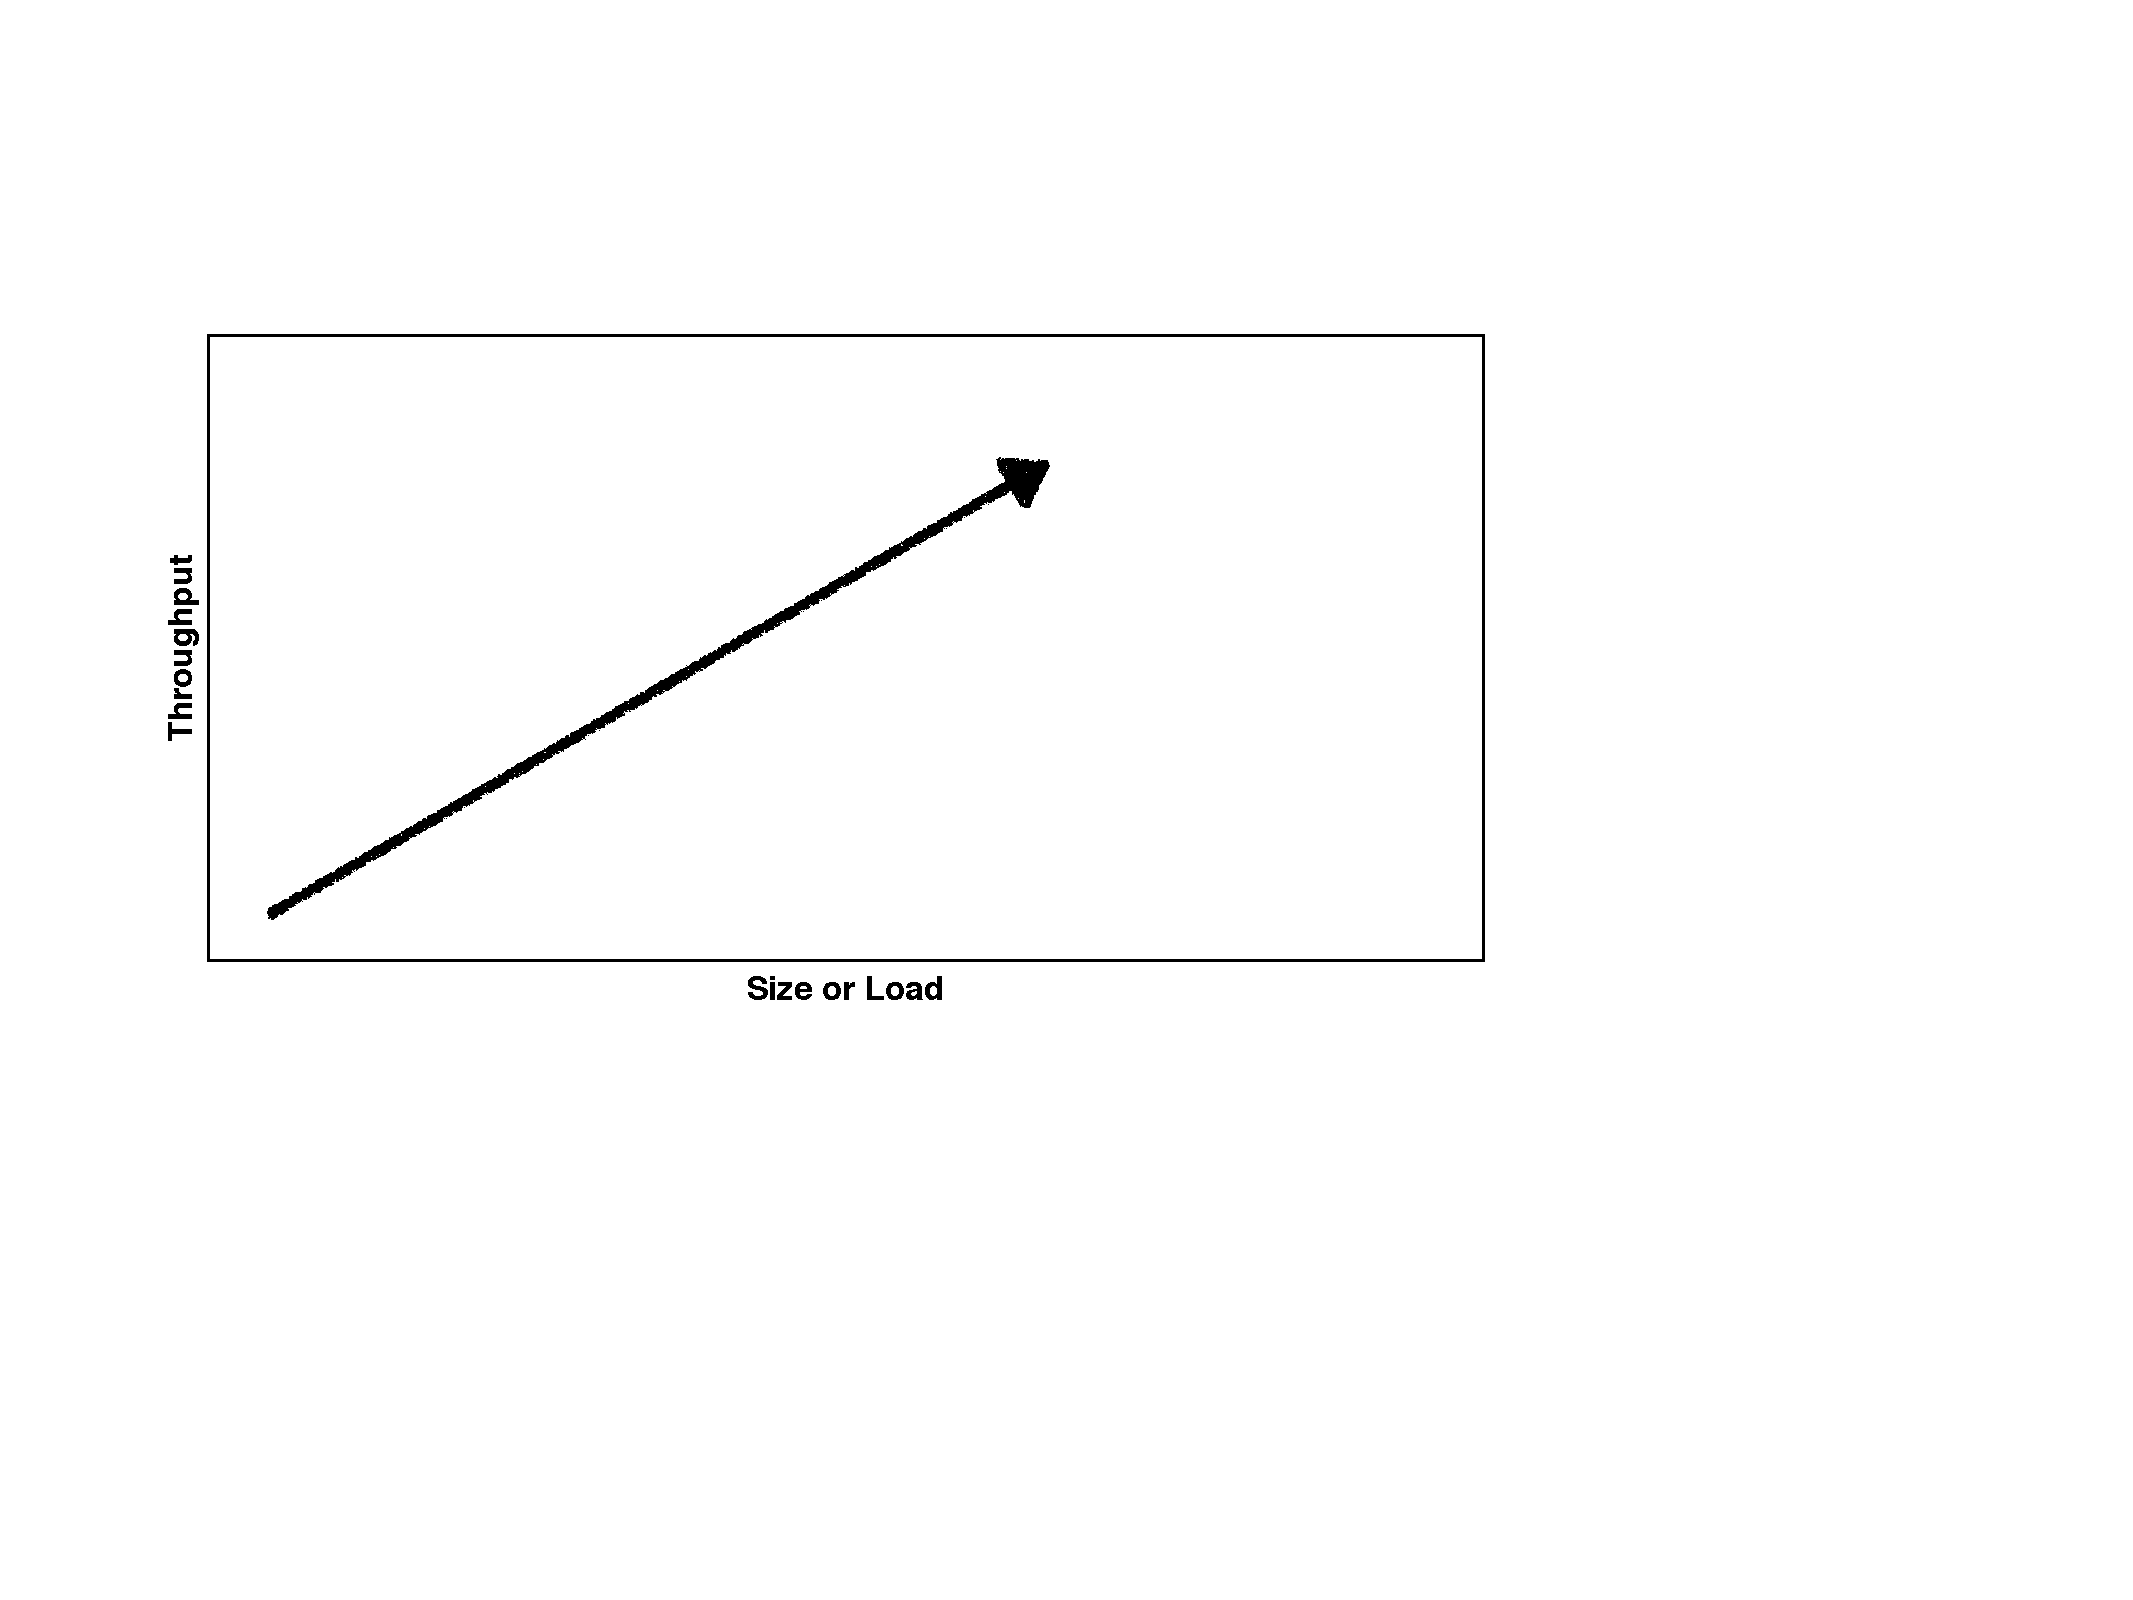
\includegraphics[width=.85\linewidth]{scalability/size-vs-load}
\end{center}

For those who are like me and need extra emphasis, I'll repeat that this is a
mathematical function, with size or load on the $X$ axis, and throughput on the
$Y$ axis. I'll make this more precise later.

\section{Linear Scalability: The Holy Grail}

In my experience, never was a marketechture slide deck created that mentions
scalability without also including the word ``linear.'' But as you might expect,
``linear scalability'' is not what people would have you believe.
\begin{center}
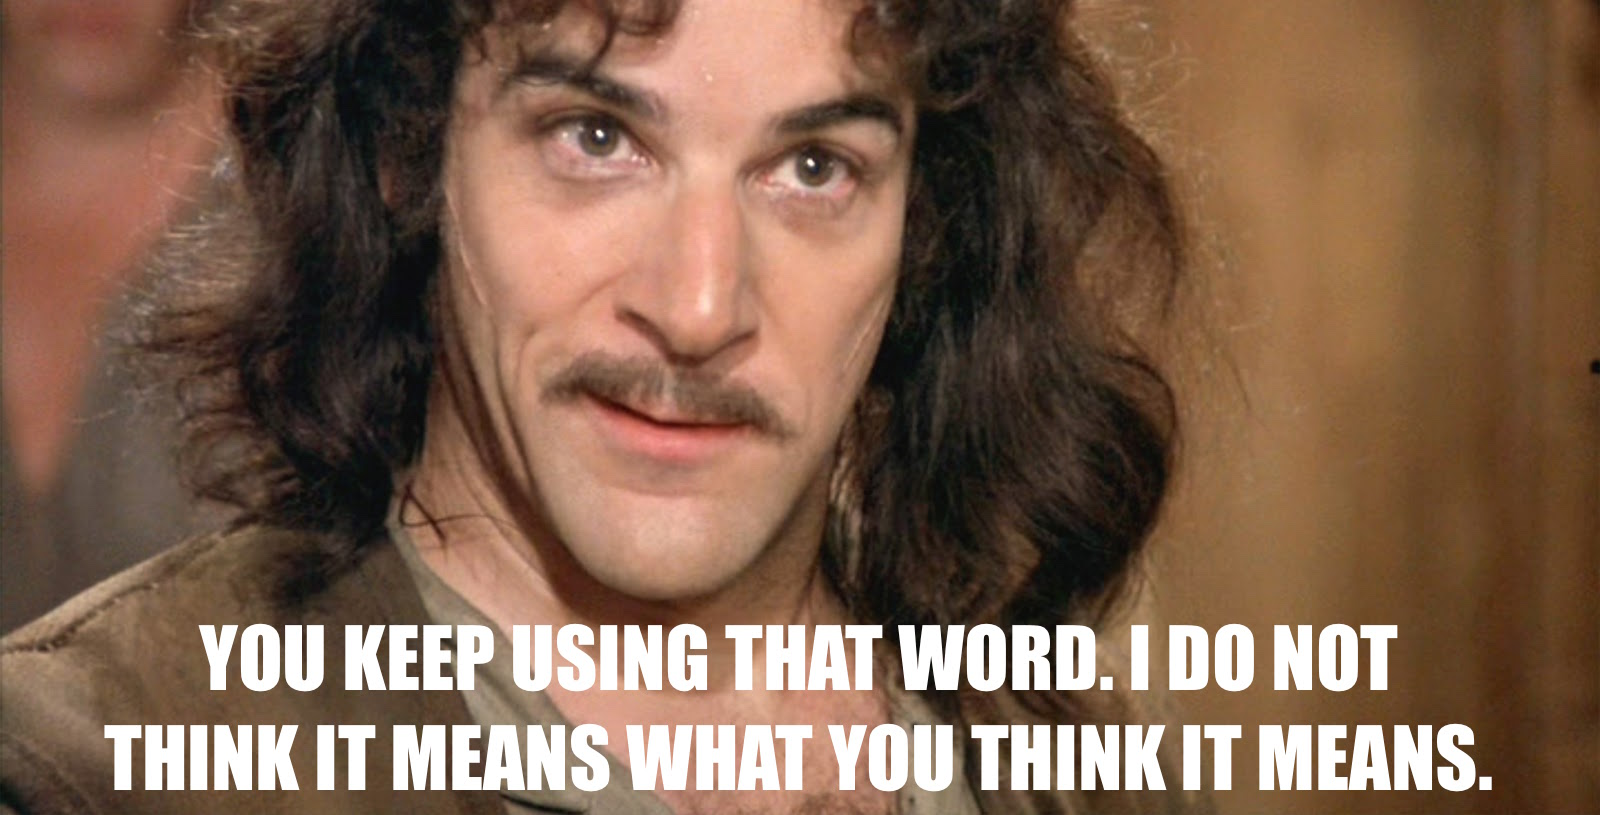
\includegraphics[width=.85\linewidth]{scalability/inigo}
\end{center}

Hand-waving claims of linear scaling usually coincide with vague definitions
of scalability, and people who know a lot about scalability rarely say the word
``linear.'' Here are a few of the misdefinitions of linear scalability I've heard:

\begin{itemize}
\item A web architect at a conference said, ``I designed our system to be
shared-nothing so it would be linearly scalable.'' He meant there was no
single resource or system imposing a hard upper limit on how many servers could
be added to the system. But he didn't really know whether his system actually
scaled linearly.
\item A technical evangelist giving a presentation about a clustered database
said, ``adding a node to the cluster adds a predictable amount of capacity.''
Predictable isn't the same as linear.
\item A sales presentation for another clustered database said the database
scaled linearly, with a ``linearity factor'' of 97\%, meaning that each
additional node increased the system's capacity by 0.97 times the amount the
previous node added. That's a curve, not a line.  (Later you'll learn how to
instantly determine the asymptotic upper bound on such a system's total
capacity.)
\end{itemize}

This may seem like a pointless rant, but it's actually important if you want to
be able to design and improve highly scalable systems.

Spotting bogus linearity claims is fun. Here are some ways
``benchmarketing'' makes systems appear linear:

\begin{itemize}
\item Show graphs without numbers, so readers can't do the math.
\item Show graphs with nonlinear axes.
\item Begin the axes, especially the $Y$ axis, at a nonzero value.
\end{itemize}

Here is a real example, redacted to protect the not-so-innocent, that employs
some of these tricks.
\begin{center}
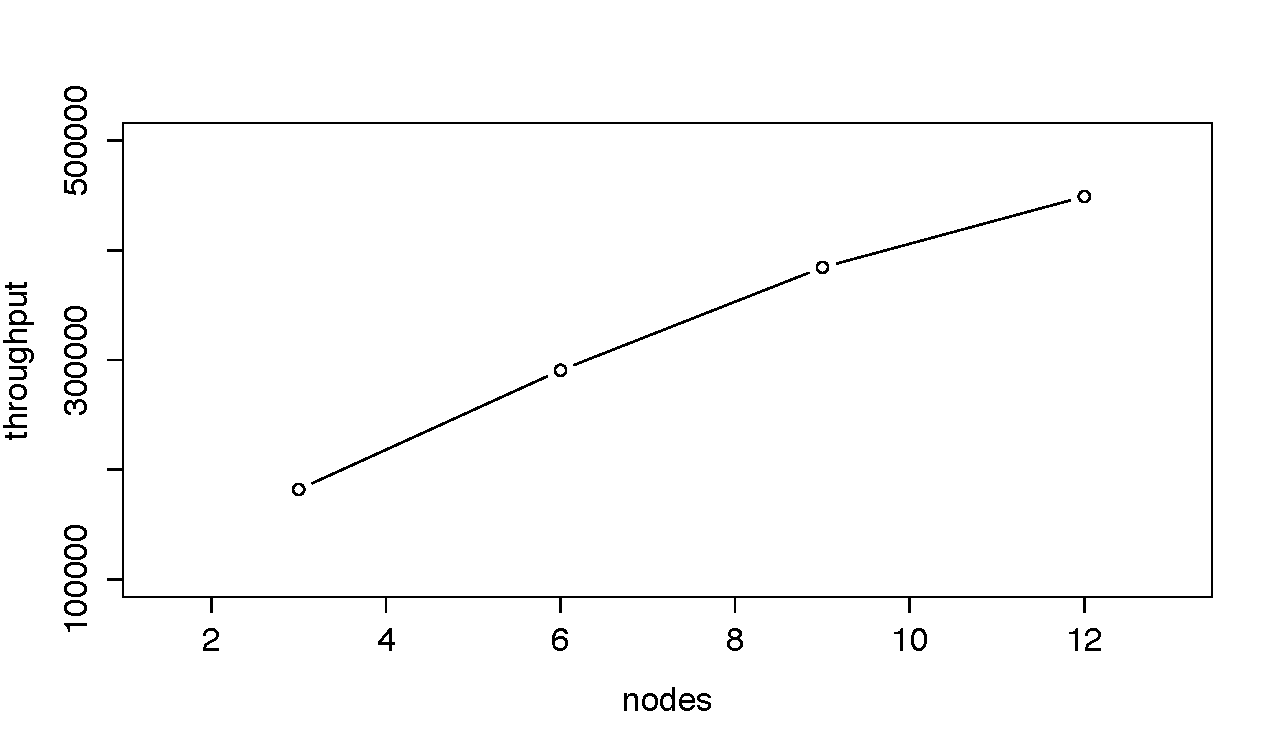
\includegraphics[width=.85\linewidth]{scalability/voltdb1}
\end{center}
Looks pretty linear, doesn't it? Yet if you do the math, it's nowhere near
linear.  It's an optical illusion, because the $X$ axis begins around
1.45 instead of zero, and the $Y$ axis starts at 100000, so you can't tell that
the chart isn't going to intersect the origin if you extend it downwards.

{\bfseries The real test of linearity is whether the transactions per second per
node remains constant as the node count increases}. The chart's original source
mentioned that throughput increased from ``182k transactions per second for 3
nodes to 449k for 12 nodes.'' The math is easy: the system achieves 60700
transactions per second per node at 3 nodes, but only 37400 at 12 nodes, which
represents a {\itshape 39\% drop in throughput} versus linear scalability.  If
it actually scaled linearly, it would achieve 728k transactions per second at 12
nodes.

Linear means linear, folks! And seemingly small amounts of nonlinearity really
matter, as you'll see later, because small sublinear effects grow very quickly
at larger scale.\footnote{In fact, they grow---wait for it---nonlinearly!}

\section{Why Systems Scale Sublinearly}

Linear scalability is the ideal, yet despite the claims, systems that actually
scale linearly are rare.  It's very useful to understand the reasons for this,
because a correct understanding of scalability, and the reasons and sources of
sublinear scaling, is the key to building more scalable systems.  That's why
it's important to be a linearity skeptic.  It's not just being pedantic.

The best way to think about linearity is as a ratio of the system's performance
at a size of 1. Neil Gunther calls this the {\itshape efficiency}.
If a system produces 1800 transactions per second with 1 node, then ideally 4
nodes produce 7200 transactions per second. That would be 100\% efficient. If
the system loses a bit of efficiency with each node and 4 nodes produce, say,
5180 TPS, then the 4-node system is only 72\% efficient:
\begin{center}
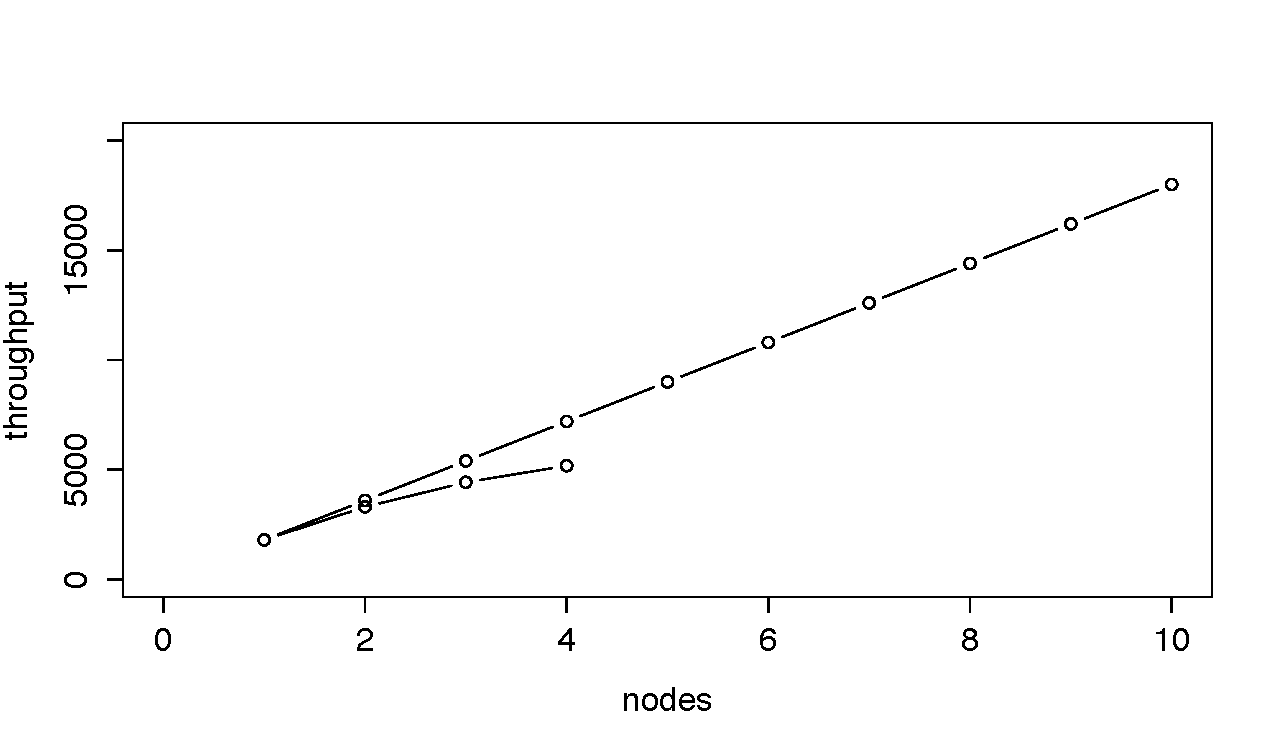
\includegraphics[width=.85\linewidth]{scalability/linear2}
\end{center}
If you do this math, you'll often be surprised at how large the 
efficiency loss is.  Graphs can be deceptive, but the numbers are quite
clear.\footnote{Drawing a linear scaling line on the graph helps, too. Without
that line, the eye tends to see the graph as more linear than it really is, and
the efficiency loss becomes less obvious.}


In the real world there's almost always some efficiency loss, and if you can
figure out why, you may be able to fix it. In fact, you've probably noticed that
real systems tend not only to fall behind linear scalability a bit, but actually
exhibit {\itshape retrograde} scalability at some point:
\begin{center}
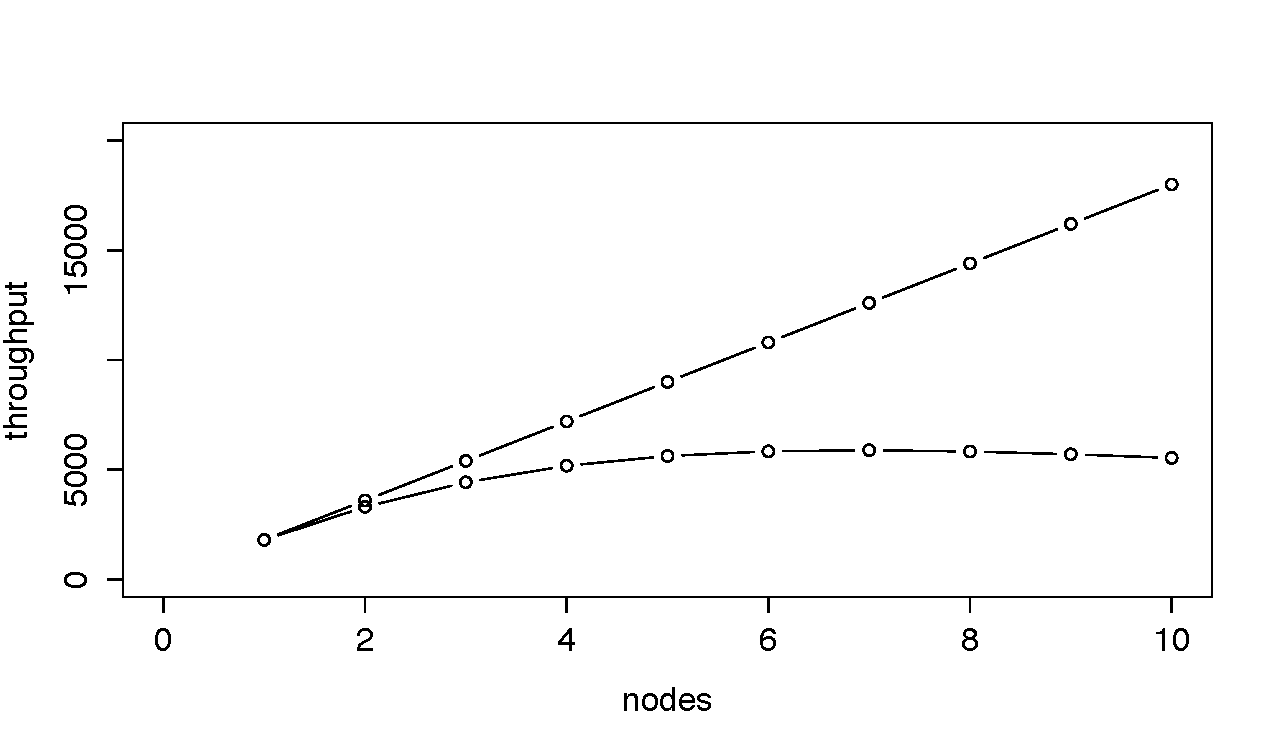
\includegraphics[width=.85\linewidth]{scalability/linear3}
\end{center}
This is quite common in the real world---you scale things up and at some point
your system starts going backwards and {\itshape losing} performance, instead of
just gaining more and more slowly. In the MySQL 5.0 days, for example, it was
common to see people upgrading from 4-core servers to 8-core servers and losing
performance.

Why does this happen? Why don't systems scale linearly, and why do they
sometimes show retrograde scalability?

According to Neil Gunther, there are two reasons: {\bfseries contention} and
{\bfseries crosstalk}. Contention degrades scalability because parts of the work
can't be parallelized and queue up, so speedup is limited. Crosstalk introduces
a coherency penalty as workers (threads, CPUs, etc) communicate to share and
synchronize mutable state. I'll explore these effects in the next section.

\section{The Universal Scalability Law}

Neil Gunther's Universal Scalability Law (USL) provides a formal definition of
scalability,\footnote{Neil Gunther originally called a slightly different form
of the USL ``superserial,'' and you may encounter this terminology, especially
in older books and papers.} and a conceptual framework for understanding,
evaluating, comparing, and improving scalability. It does this by modeling
the effects of linear speedup, contention delay, and coherency delay due to
crosstalk.

Let's see how this works, piece by piece. An ideal system of size 1
achieves some amount $\lambda$ of throughput $X$, in completed requests per
second. Because the system is ideal, the throughput doubles at size $N$=2, and so
on. This is perfect linear scaling:
\begin{equation}
X(N) = \frac{\lambda N}{1}
\label{linear}
\end{equation}

The $\lambda$ parameter defines the slope of the line. I call it the {\itshape
coefficient of performance}. It's how fast the system performs in the special
case when there's no contention or crosstalk penalty.
Here are two ideal systems, with $\lambda$ of 1800 and 800, respectively.
\begin{center}
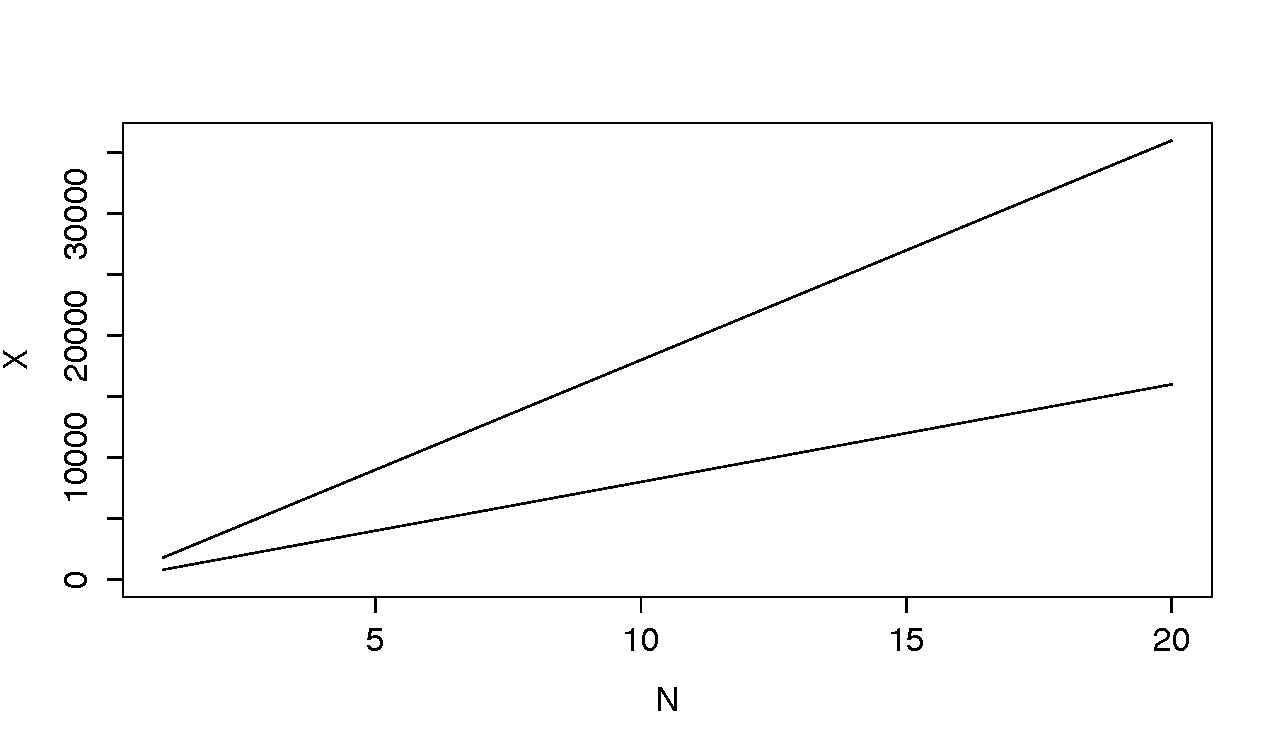
\includegraphics[width=.85\linewidth]{scalability/ideal-linear}
\end{center}

Note that every linearly scalable system is just as scalable as any other,
regardless of the slope of the line. They have different performance but
identical scalability characteristics: speedup is unlimited. 

Contention appears in most systems\footnote{Including teams of people. This is a
joke but it's also true in the queueing sense.} at
some point, for example as a final stage of assembling the multiple outputs
generated in parallel into a single final result. As parallelization increases,
contention becomes the limiting factor. This is codified in
\href{https://en.wikipedia.org/wiki/Amdahl\%27s\_law}{Amdahl's Law}, which
states that the maximum speedup possible is the reciprocal of the serial
fraction. If I add a term to the denominator expressing the serial fraction of
the work, multiplied by $\sigma$, the coefficient of contention, it becomes
Amdahl's Law:
\begin{equation}
X(N) = \frac{\lambda N}{1 + \sigma(N-1)}
\label{amdahl}
\end{equation}

A system with contention will
asymptotically approach a ceiling on speedup. If $\sigma$ is .05, for example,
the speedup approaches 20. Let's see that graphically:
\begin{center}
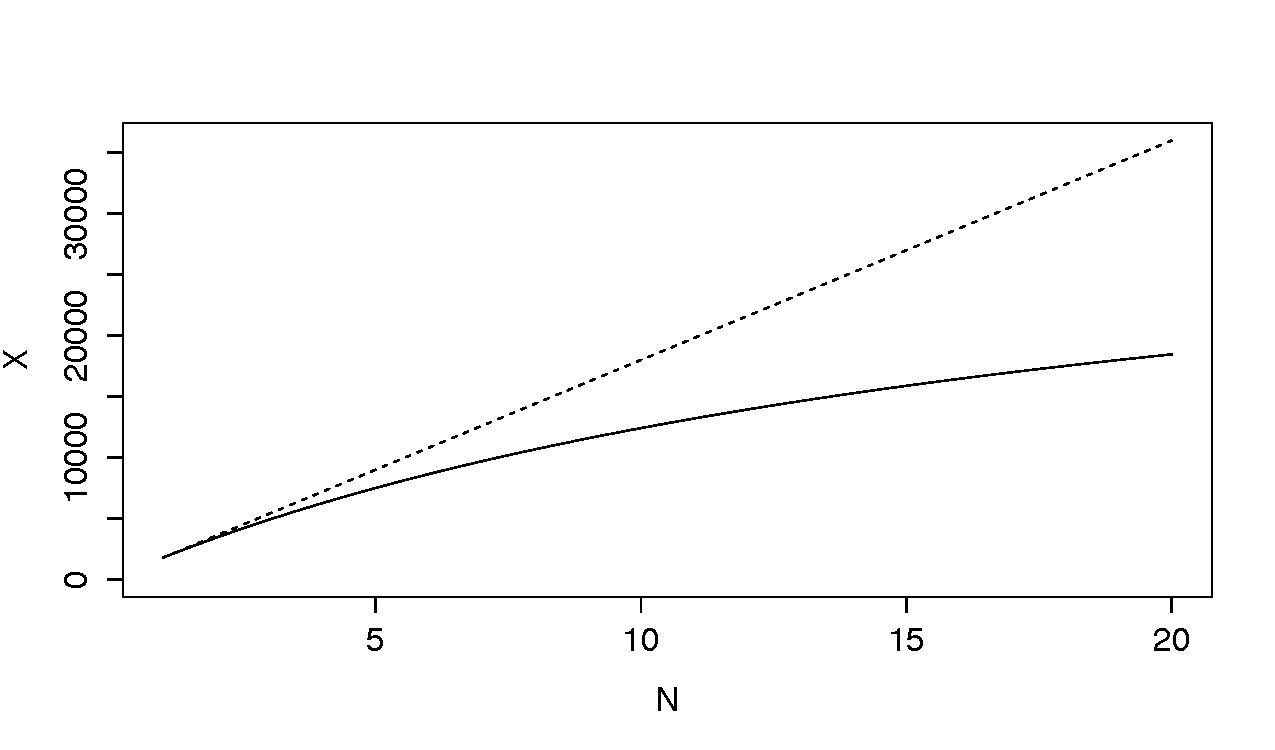
\includegraphics[width=.85\linewidth]{scalability/amdahl}
\end{center}

Remember the system I mentioned earlier, which a salesperson claimed to have
97\% scalability with each additional node? That's 3\% loss of scalability per
node, so this system will never achieve a speedup factor of more than 33, no
matter how many nodes it has.

The last bit is the crosstalk penalty, also called the consistency or coherency
penalty.\footnote{I call it crosstalk because in my opinion it's the best
description of the pairwise communication that must occur to make distributed
data or other shared resources consistent or coherent.} Crosstalk potentially
happens between each pair of workers in the system (threads, CPUs, servers,
etc).  You probably remember that the number of edges in a fully connected graph
is $n(n-1)$.  The USL represents the amount of crosstalk with another term, multiplied
by $\kappa$, the coefficient of crosstalk:
\begin{equation}
X(N) = \frac{\lambda N}{1 + \sigma(N-1) + \kappa N(N-1)}
\label{usl}
\end{equation}

Equation \ref{usl} is the Universal Scalability Law.

The crosstalk penalty grows fast. Because it's quadratic,\footnote{The cost of
$n(n-1)$ is $\mathcal{O}(n^2)$. If you're not familiar with it,
\href{https://www.vividcortex.com/blog/2013/10/23/big-o-notation-made-simple/}{this
blog post introduces Big-O notation}.} eventually it grows faster than the
linear speedup of the ideal system we started with, no matter how small $\kappa$
is. That's what makes retrograde scalability happen, as you can see in the
following chart:
\begin{center}
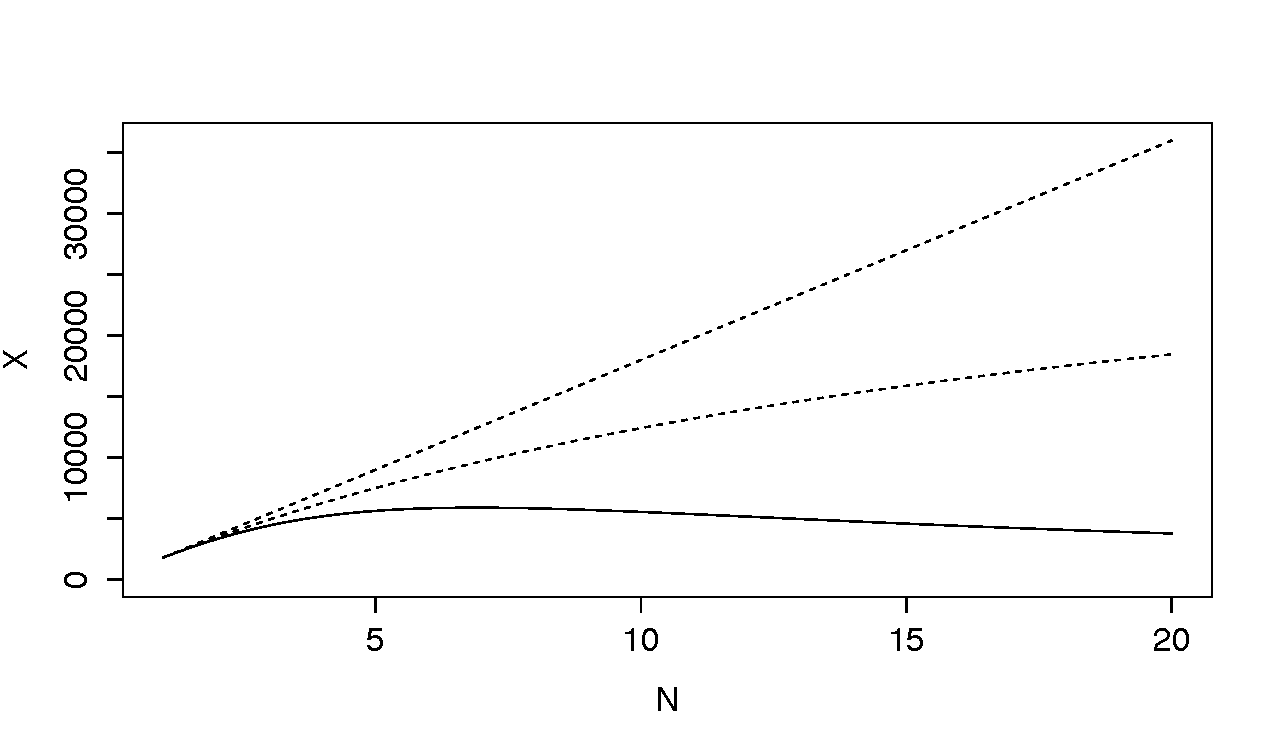
\includegraphics[width=.85\linewidth]{scalability/usl}
\end{center}

That's the Universal Scalability Law in all its glory.  This plot has the same
parameters as the ones I showed before, where a system of size 4 produced only
72\% of its ideal output. That system has 5\% contention and 2\% crosstalk,
and now that I've plotted it out to size 20 you can see it's embarrassingly
inefficient.  In fact, I should have given up trying to scale this system after
size 6 or so.

This shows visually how much harm a ``small amount'' of nonlinearity can do in
the long run.  Even very small amounts of these damaging coefficients will
create this effect sooner or later (mostly sooner). This is why it's rare to
find clustered systems that scale well beyond a couple dozen nodes or so.
If you'd like to experiment with this interactively, I've made a graph of it at
\href{https://www.desmos.com/calculator/2l0jcjmsxn}{Desmos}.

\section{The USL's Relationship to Queueing Theory}

The USL is closely related to queueing theory. Neil Gunther proved that it's
equivalent to synchronous repairman queueing. If you're not familiar with
queueing theory, I wrote an approachable introduction called
\href{https://www.vividcortex.com/resources/queueing-theory/}{Everything You
Need To Know About Queueing Theory}.

The two causes of sublinearity have important relationships to queueing theory.
Contention, the first term I added to the denominator to obtain Amdahl's Law,
expresses the penalty from queueing delay that occurs when there is competition
for shared resources---the servers (in the queueing theory sense) that process
work from queues.

The queue length is {\itshape nonlinear} with respect to utilization and
therefore to offered load. Queueing theory is confusing and counterintuitive! As
the queues lengthen, the queueing delay lengthens in direct proportion.

As you probably know, queueing theory treats service time---the amount of time
it takes to complete a job after it leaves the queue and enters service---as
independent of utilization or queueing. The job takes as long as needed to
execute all the instructions, whether the server is busy or idle. The customer's
total wait time at a busy server is longer only because of queueing delay.

Coherency penalty, which comes from crosstalk, actually expresses an {\itshape
increase in service time} that is not due to queueing delay. As the system has
to do more crosstalk to synchronize mutable shared state, the jobs take longer
and longer. This is {\itshape not} due to queueing---the job is already out of
the queue and in service.

These effects are clearly visible in the USL when it enters the region of
retrograde scalability. An increase in service time is the only thing that can
explain retrograde scalability. If the service time remained constant,
throughput would be a flat line. Queue length and queue wait time cannot explain
retrograde scalability; queueing can only cap throughput, not decrease it.

\newpage
\section{Measuring Scalability}

To recap, at this point we've figured out the right dimensions for a formal model
of scalability that seems to behave as we know real systems behave, and examined
Neil Gunther's USL, which fits that framework well and gives us an equation for
scalability. (Are you excited yet?)

Now what can you do with it?

Great question! It turns out you can do a lot of extremely useful things with the
USL.  Unlike a lot of models of system behavior, this one is actually practical
to apply in the real world. That's the real genius of it, in fact. Not only is
the equation uncomplicated, but the variables it describes are easy to get most
of the time.

I use the USL mostly for modeling system scalability, by working backwards from
observed system behavior and estimating the likely coefficients. To accomplish
this, you need a set of measurements of the system's load or size (usually
concurrency or node count) and the corresponding throughput. Then you {\itshape
fit} the USL to this dataset, using nonlinear least squares regression. This is
a statistical technique that finds the optimal coefficient values in order to
calculate a best-fit line through the measurements. The result is values for
$\lambda$, $\sigma$, and $\kappa$.

If you're reading about the USL in Neil Gunther's books, he takes a different
approach. First, he doesn't use regression to determine $\lambda$, he assumes
that you can measure it in a controlled way at $N=1$. (I've often found that's
not true for me.) Secondly, there are a couple of different forms of the
USL---one for hardware scaling and one for software scaling---which are the same
equation, but with different parameters. For simplicity I'm treating them as
interchangeable. I will write a bit more about this later.

Examples of systems I've analyzed with the USL include:

\begin{itemize}
\item Black-box analysis of networked software simply by observing and
correlating packet arrivals and departures, looking at the IP addresses, port
numbers, and timestamps. From this I computed the concurrency by averaging the
amount of time the system was busy servicing requests over periods of time. The
throughput was straightforward to get by counting packet departures.
\item MySQL database servers. Some of its \texttt{SHOW STATUS} counters are
essentially equivalent to throughput and concurrency.
\item Linux block devices (disks) by looking at \texttt{/proc/diskstats}, from
which you can get both instantaneous and average concurrency over time deltas,
as well as throughput (number of I/Os completed).
\item Lots and lots---and lots---of benchmark results.
\end{itemize}

I've built a variety of tools to help clean, resample, and analyze the data
before arriving at satisfactory results. Most of them were commandline, though
these days I use R more than anything else. This is an important topic:
you will get dirty data, and that will
make your results less useful. You need to visualize both in scatterplot form as
well as in time-series form and ensure you're working with a relatively
consistent set of data. You can remove individual points or trim the time range
you use, and you may need to experiment with averaging the data over time to get
good results.

As for the R code, I'll give a little bit of a quickstart to show the
soup-to-nuts approach.  You'll save the data into a delimited file, with column
headers \texttt{size} and \texttt{tput}. Then you'll load this into a variable
in R and regress it against the USL.

Here's a complete sample, based on a
\href{https://www.percona.com/docs/wiki/benchmark:cisco:scale:start}{benchmark}
that Vadim Tkachenko ran on a Cisco server:

\begin{verbatim}
size tput
1 955.16
2 1878.91
3 2688.01
4 3548.68
5 4315.54
6 5130.43
7 5931.37
8 6531.08
9 7219.8
10 7867.61
11 8278.71
12 8646.7
13 9047.84
14 9426.55
15 9645.37
16 9897.24
17 10097.6
18 10240.5
19 10532.39
20 10798.52
21 11151.43
22 11518.63
23 11806
24 12089.37
25 12075.41
26 12177.29
27 12211.41
28 12158.93
29 12155.27
30 12118.04
31 12140.4
32 12074.39
\end{verbatim}

Save that data into a file, say, \texttt{benchmark.txt}. Then load it and run the following commands:

\begin{verbatim}
benchmark <- read.csv("/path/to/benchmark.txt", sep="")
usl <- nls(tput ~ lambda*size/(1 + sigma * (size-1) + kappa * size *
   (size-1)), benchmark, start=c(sigma=0.1, kappa=0.01, lambda=1000))
summary(usl)
sigma <- coef(usl)['sigma']
kappa <- coef(usl)['kappa']
lambda <- coef(usl)['lambda']
u=function(x){y=x*lambda/(1+sigma*(x-1)+kappa*x*(x-1))}
plot(u, 0, max(benchmark$size)*2, xlab="Size", ylab="Throughput", lty="dashed")
points(benchmark$size, benchmark$tput)
\end{verbatim}

The results are as follows:
\[
\begin{array}{ll}
			\lambda&995.6486 \\
     \sigma & 0.02671591 \\
			       \kappa & 0.0007690945 \\
\end{array}
\]

Note the extremely small value for $\kappa$ which nonetheless degrades
scalability before $N$ becomes very large. Here's the resulting plot:
\begin{center}
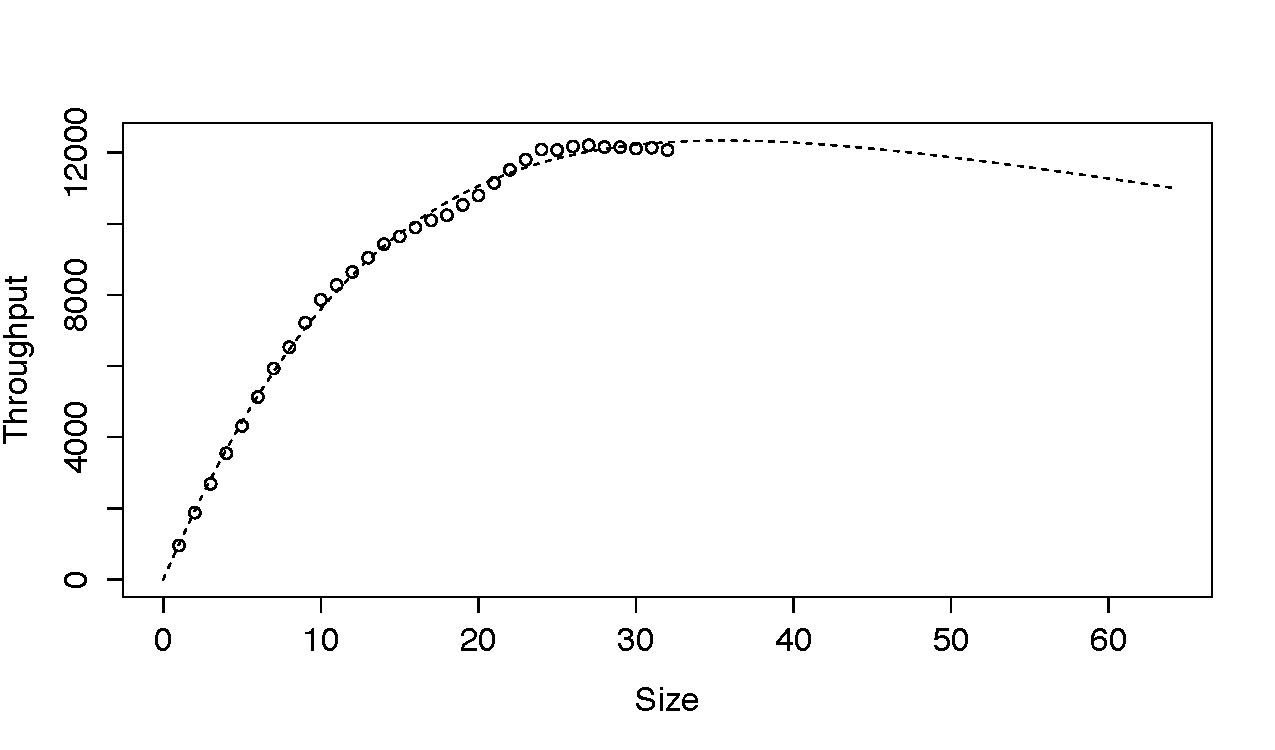
\includegraphics[width=.85\linewidth]{scalability/cisco}
\end{center}

If you're an R user, that's probably all you need to get going. You really
should do more diligence, such as checking the $R^2$ value of the fit. But
instead of doing all this work manually (which you can certainly do if you
want), I suggest trying the
\href{https://cran.r-project.org/web/packages/usl/}{USL package from CRAN}. It
has many features built in, although it does have some limitations.

One final thing: if the $\kappa$ coefficient has a nonzero value, the function
has a maximum. You can find the size of the system at that maximum as follows:
\begin{equation}
N_{max} = \left \lfloor \sqrt{\frac{1-\sigma}{\kappa}} \right \rfloor
\label{n_max}
\end{equation}

You can find the maximum predicted throughput by plugging $N_{max}$
into Equation \ref{usl}. Doing so with the coefficients in this example
predicts the system's throughput will increase until $N=35$, which in this case
means 35 threads, and the peak throughput will be 12341 queries per second. It
also found $\lambda$, the throughput at $N=1$, to be 995 QPS, which is close to
the actual value of 955.

It's always interesting to use the USL on a subset of the performance data, such
as the first third or so, to see how well it predicts the higher $N$ values.
This can be quite educational.

Note that you should have at least half a dozen or so data points in order to
get good results in most circumstances. In practice I usually try to capture at
least a dozen for benchmarks, and more---often thousands---when analyzing
systems that aren't in a controlled laboratory setting.

\section{Modeling Response Time}

What is the relationship between scalability and performance?  Throughput and
latency are two common ways to describe and measure performance. Most benchmarks
measure overall system throughput, and claims of performance are almost always
in throughput terms: ``a million transactions per second,'' and so on.
Benchmarks usually define performance as how much work the system can do.

On the other hand, users care mostly about the performance of individual
requests. For example, a user's opinion of website performance is based entirely on
how quickly pages load and render.  From this viewpoint, as Cary Millsap says,
{\itshape performance is response time}.

Which view is right? Both. System performance is measured in throughput, and
request performance is measured in latency. And because throughput and latency
are related, scalability also has dual meanings: the system's ability to
complete more work at larger sizes, and its response time characteristics.

I've shown that the USL can model and forecast how size affects throughput. Can
it also model latency? Yes, it can when the independent variable is concurrency,
because of a relationship called Little's Law:
\begin{equation}
N = X R
\label{littles_law}
\end{equation}

Little's Law says that the mean number of requests resident in a system is
equal to the throughput times the mean response time. This relationship is
valid for stable systems, in which all requests eventually complete.

If you use Little's Law to solve the USL for response time as a function of
concurrency, the result is a quadratic function:

\begin{equation}
R(N)=\frac{1+\sigma(N-1)+\kappa N(N-1)}{\lambda}
\label{r_n}
\end{equation}

This means that response time\footnote{{\itshape Mean} response time. You could
use queueing theory to add nuance, such as the probability that any given
request needed to wait more than a set amount of time.} is related to the square
of concurrency.  Of course, just as with the USL, if the $\sigma$ or $\kappa$
coefficients are zero, the equation is simplified, removing the causes of
nonlinear behavior. One of the nice things about Equation \ref{r_n} is that you
can now see the effects of contention (linearly increasing queueing delay) and
coherency (quadratically increasing service time) on residence time.  Here's the
same data I used previously, now inverted and used to predict response time. The
dashed lines show linear and Amdahl response time scaling for the same
$\lambda$:
\begin{center}
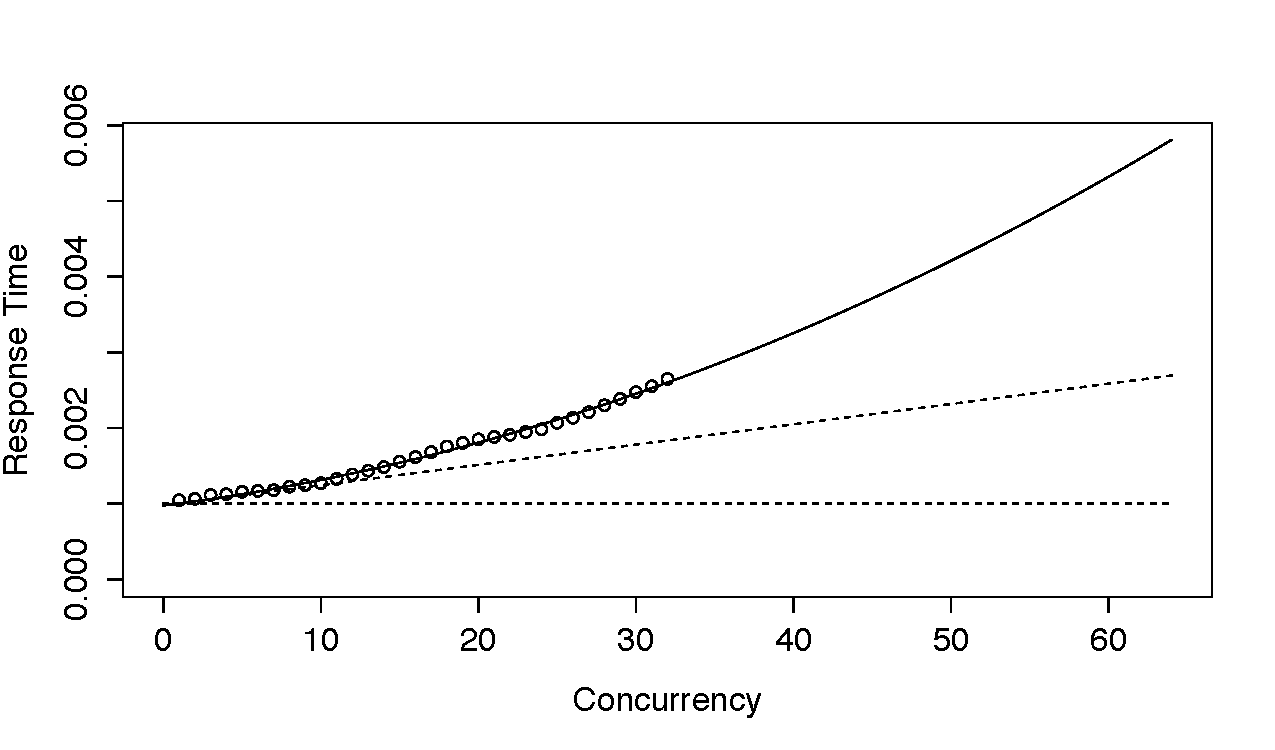
\includegraphics[width=.85\linewidth]{scalability/cisco-tput}
\end{center}

Be careful not to confuse this chart with another famous ``hockey stick'' chart,
that of response time versus utilization, which is familiar from queueing
theory:
\begin{center}
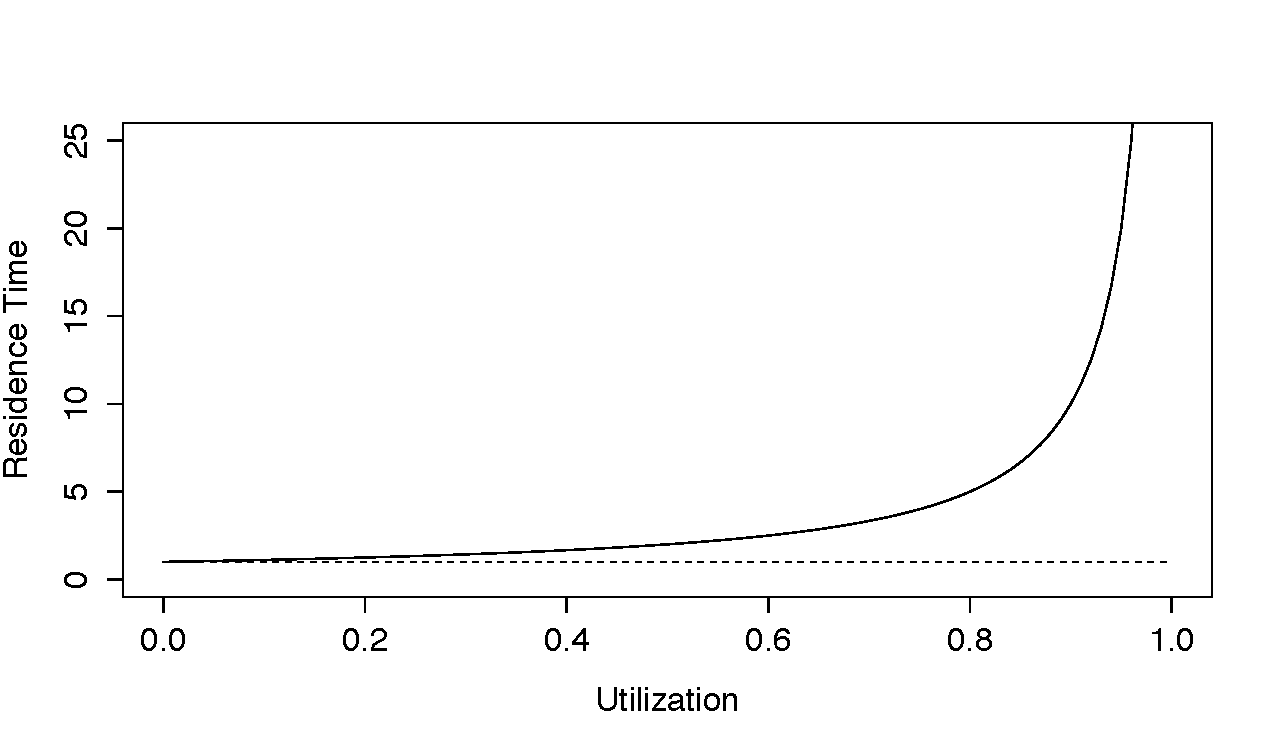
\includegraphics[width=.85\linewidth]{scalability/hockey}
\end{center}

The difference is that one chart uses utilization as the independent variable,
which ranges only from 0 to 1, whereas the other uses concurrency, which has no
fixed upper limit.\footnote{The relationship between concurrency and utilization
is nonlinear; according to the USL, it is quadratic.}

Little's Law also lets you rearrange the USL in terms of the relationship
between throughput and latency, which is useful for a few reasons. It lets you
model scalability and performance in these dimensions, it helps build intuition
about what happens when systems don't scale linearly,  and it relates the USL to
queueing theory visually in an important way.
I'll begin by showing response time as a function of throughput, which is a
common way I've seen people (and vendors) plot it. Beginning with a linearly
scalable system,
\[
R(X) = \frac{1}{\lambda}
\]

Response time is constant. Adding a positive $\sigma$ coefficient\footnote{I am
omitting step-by-step solutions for brevity, but Wolfram Alpha can show this if
you're curious. The easiest way is to solve the USL for $R$ as a function of
$X$ and simplify.} makes it an exponential function:
\begin{equation}
R(X) = \frac{\sigma - 1}{\sigma X - \lambda}
\label{amdahl_r_x}
\end{equation}

Response time goes to infinity as throughput approaches $\lambda/\sigma$. The
following plots are generated with the parameters $\sigma=\kappa=.06,
\lambda=40$:
\begin{center}
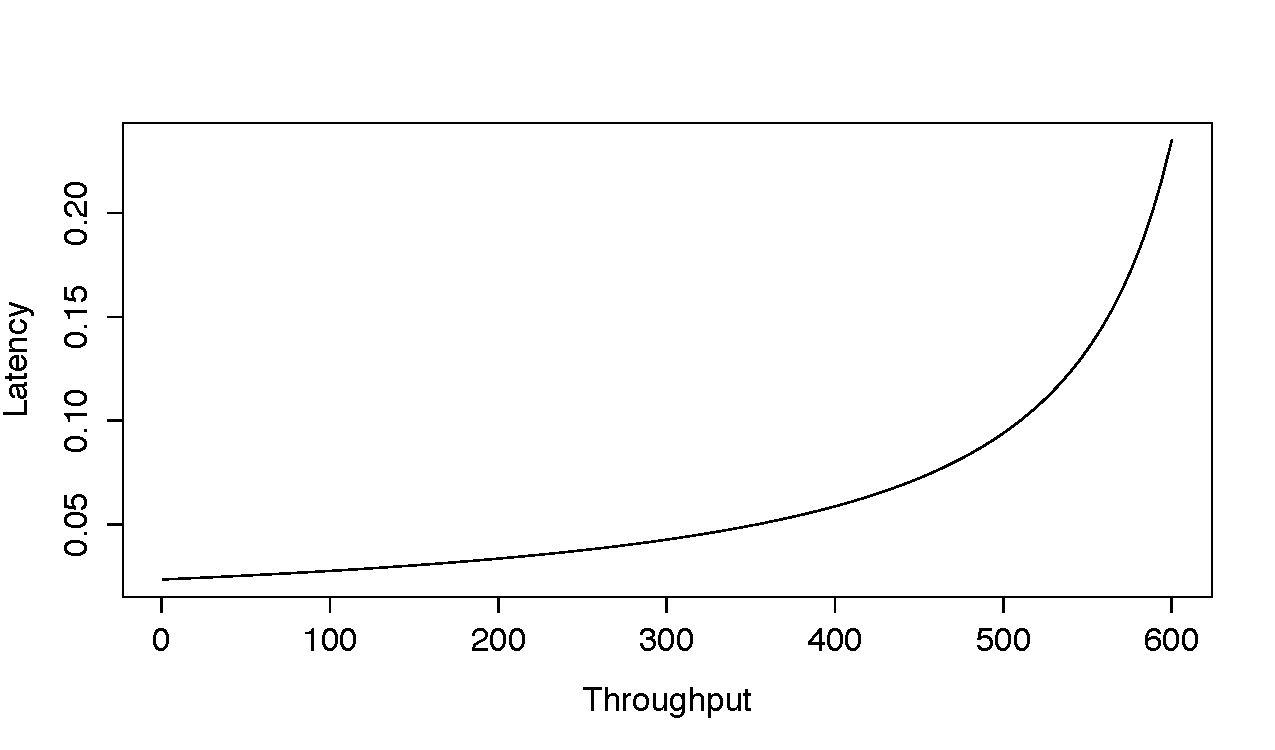
\includegraphics[width=.85\linewidth]{scalability/r-function-x-amdahl}
\end{center}

The response time curve's relationship to the queueing theory response time
curve (which is in terms of $\rho$) is more obvious now. What happens when you
add coherency to the equation? The equation has multiple solutions.  Instead of
merely lifting away from the response-time line, it folds back on itself like a
``nose.'' The solution for the lower portion of the curve is as follows:
\begin{equation}
R(X)=\frac{-\sqrt{X^2(\kappa^2+2\kappa(\sigma-2) + \sigma^2)+2\lambda X(\kappa-\sigma)+\lambda^2}+\kappa X+\lambda-\sigma X}{2\kappa X^2}
\label{r_x_lower}
\end{equation}

The other solution is simply the negative. Here's a plot of both:
\begin{center}
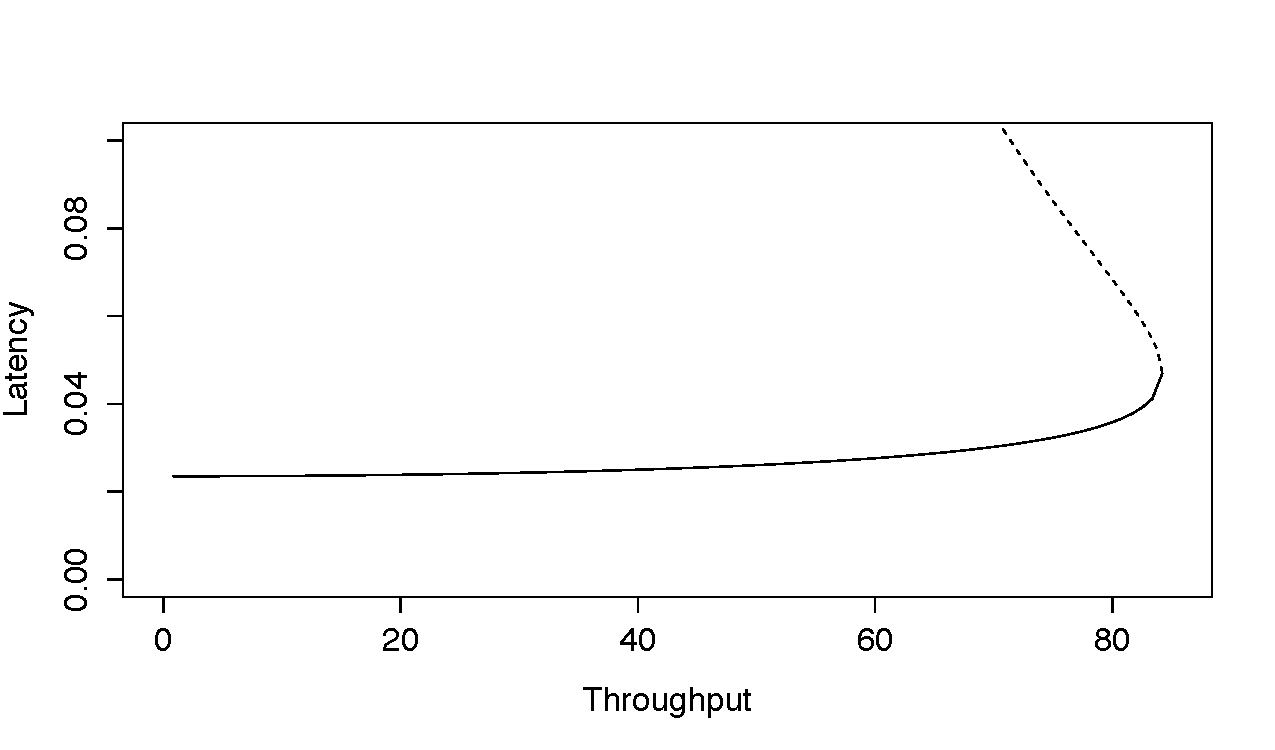
\includegraphics[width=.85\linewidth]{scalability/nose-equation}
\end{center}

%Here is a plot of the same points as previously, with axes transposed:
%illustrate:
%\begin{center}
%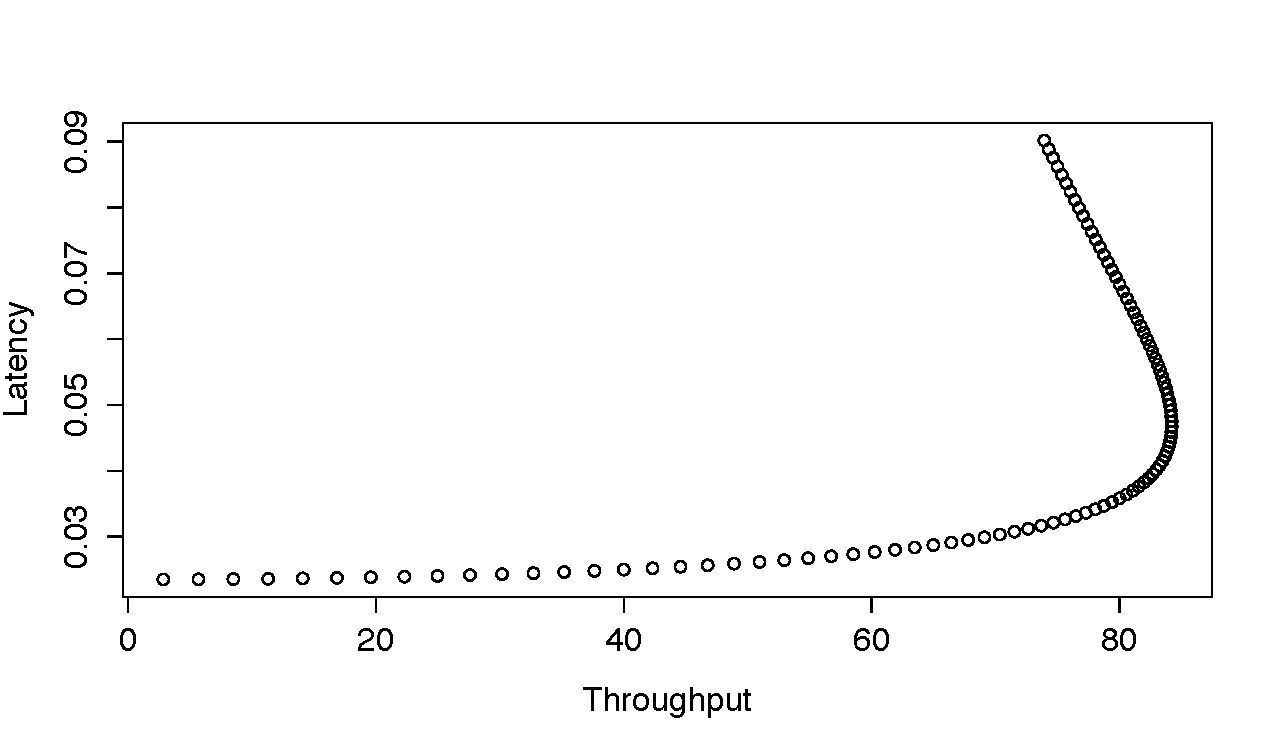
\includegraphics[width=.85\linewidth]{scalability/nose}
%\end{center}

As you can see, this is not strictly a function of $X$, since a single $X$ value
can map to two values of $R$ due to the multiple solutions. {\itshape Response
time is not a function of throughput if $\kappa$ is nonzero.} The inverse is
actually true---given a target latency, you can uniquely identify the throughput
at which it will occur:
\begin{equation}
X(R)=\frac{\sqrt{\sigma^2+\kappa^2+2\kappa(2\lambda R+\sigma-2)}-\kappa+\sigma}{2\kappa R}
\label{x_r}
\end{equation}

Here's a plot of that:
\begin{center}
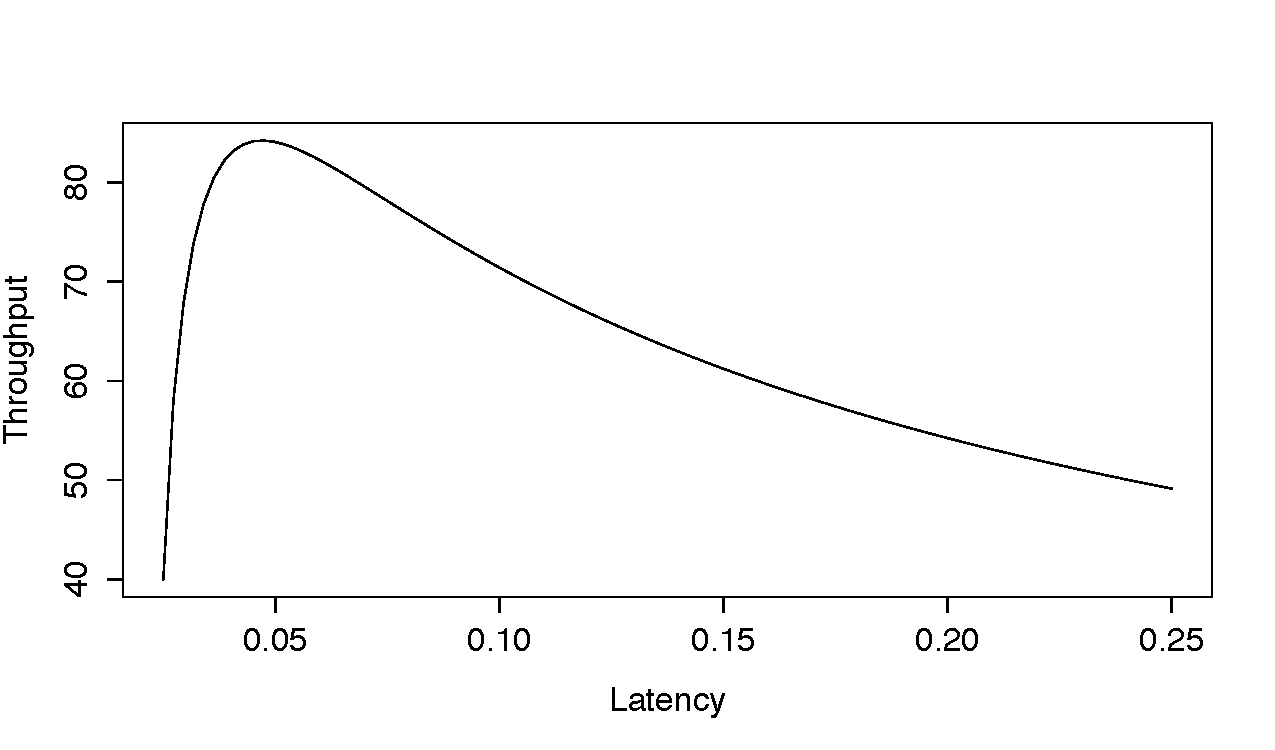
\includegraphics[width=.85\linewidth]{scalability/x-function-r}
\end{center}

Real systems actually do behave this way. The maximum throughput in that chart,
of course, is the same as the maximum throughput in the USL function with the
same parameters. And the latency at which it occurs corresponds exactly to
$N_{max}$ from Equation \ref{n_max}. The relationship between these quantities
is simply Little's Law.

You can use Equation \ref{x_r} to model scalability and performance in terms of
latency, just as you use the USL to model it in terms of concurrency or size.
For example, referencing the Cisco benchmark again, you can see in a
scatterplot that the system has exceeded the point of diminishing returns and is
climbing up the nose:
\begin{center}
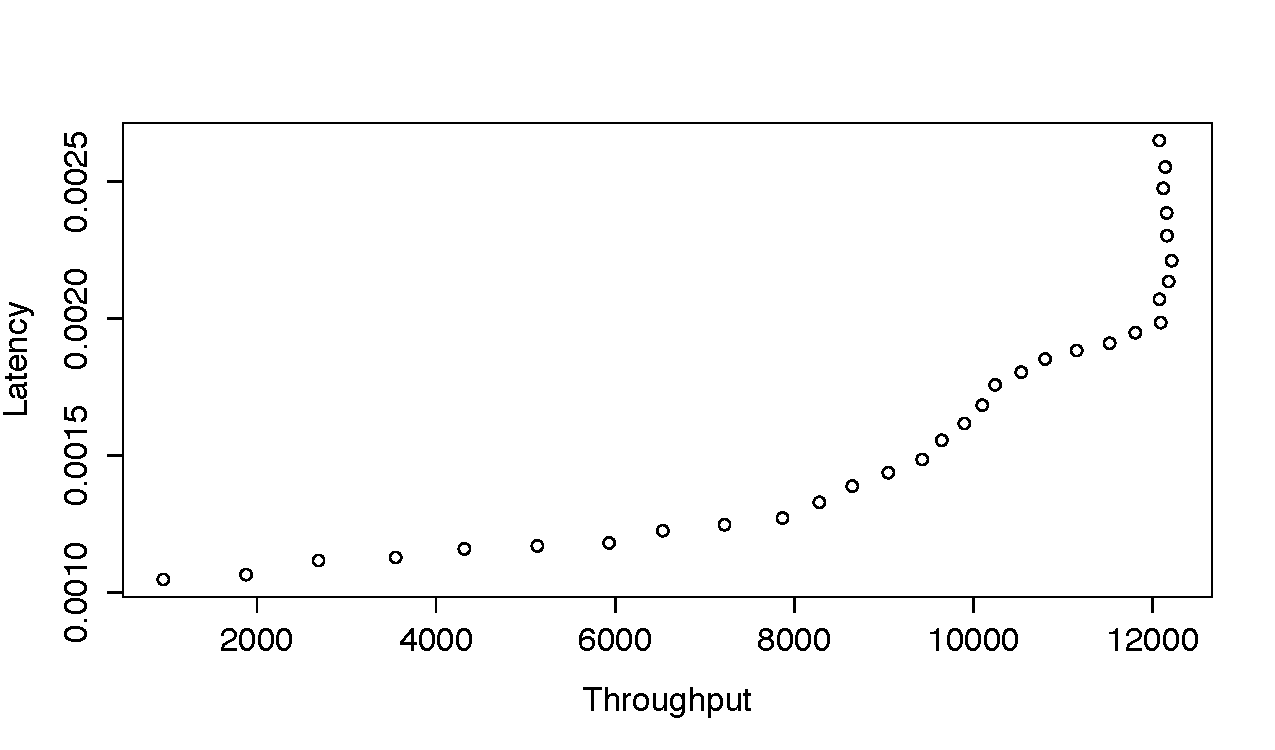
\includegraphics[width=.85\linewidth]{scalability/not-a-function}
\end{center}

This isn't a single function of throughput, as I said previously. That is why
you can't model it with a curve such as a parabola or an exponential function.
The lower portion of the nose might {\itshape look like} an exponential curve,
but it isn't. It's quite different.  Here's what happens if you try to fit an
exponential function, such as Equation \ref{amdahl_r_x},
through the benchmark's results. It way underestimates how fast latency grows.
\begin{center}
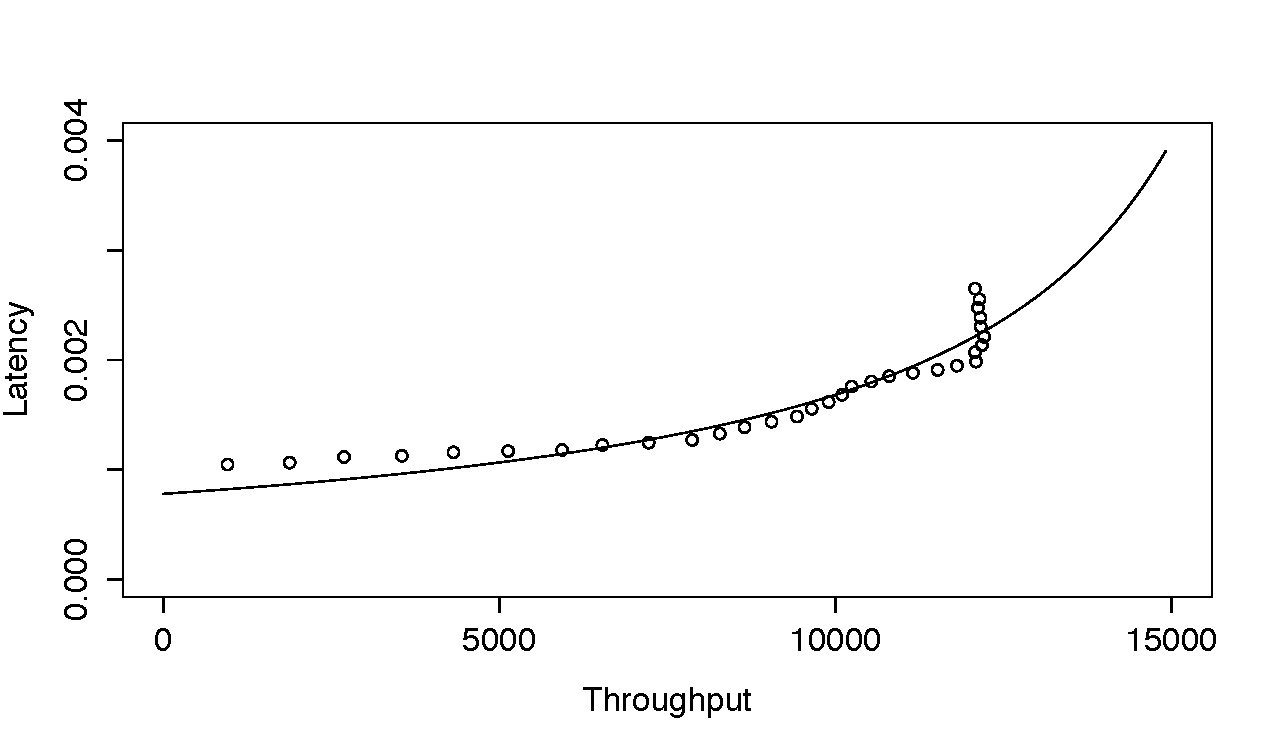
\includegraphics[width=.85\linewidth]{scalability/cisco-x-v-r-amdahl}
\end{center}

Most people probably never will see a system curve around the tip of the nose
and start climbing backwards ``in the wild,'' because the system's performance
becomes extremely bad.  This usually won't happen in production because the
load-generating systems (and users) are finite and don't continue adding work to
the system you're measuring. For example, you likely will not see this happen in
a production database because all the Apache workers get busy waiting for
queries to finish, so they can't issue more.

If you won't see it in production, then where will you? Easy---in benchmarks,
where you can fire up a practically unlimited number of driver threads. I've
seen it in many benchmarks myself.

If production systems won't climb around the tip of the nose, does the nose's
precise equation matter? Yes, because if you want to model how response time
behaves as it approaches the nose, you need the right model. With the wrong
model you'll be way off when doing things like capacity planning, which
coincidentally is the next topic I want to cover.

\section{Capacity Planning with the USL}

``How much load can this system sustain?'' is a common question in capacity
planning. The practical purpose is usually something like the following:

\begin{itemize}
\item How soon will the system begin to perform badly as load increases?
\item How many servers will I need for the expected holiday load?
\item Is this system close to a point of failure?
\item Are we overprovisioned? By how much?
\end{itemize}

Capacity planning is often a difficult problem because it's hard to tell what a
system's true capacity is. The USL can help you estimate this.

Conventional ways to determine system capacity are often difficult, expensive,
and don't give results you can really believe in. For example, you can set up
load tests, but it takes a lot of work and time, and the results are suspect
because the workload is always artificial in some way.

You can also run benchmarks, but most benchmarks are pretty useless for
predicting a system's usable capacity. In addition to being an artificial
workload, they push a system to its maximum throughput and beyond. As I
mentioned, it's rare for benchmarks to be run by people who understand the
importance of latency. But when I do see benchmarks that measure latency
percentiles, the systems almost always perform very badly at their peak
throughput.\footnote{This is a problem with the way benchmarks are usually
designed, in my opinion. I'd really prefer for the benchmark system to be
intelligent enough to back off and reduce pressure on the system under test if
it violates a service level objective (SLO).  Ideally, this is defined as a
quantile, such as 99th percentile latency less than 10ms.  A smart benchmark
would throttle load, eventually finding a longterm stable arrival rate at which
the SUT can consistently perform well.}

Another way I've tried to predict system capacity in the past is with queueing
theory, using the Erlang C formula to predict response time at a given
utilization.  Unfortunately, this requires that you know service times,
which are often impossible to obtain. You can measure total response time, but
that includes waiting time in the queue, so it's not the same thing as the
service time. The utilization is also often deceptive, because the real
utilization of the resources you're trying to model can be difficult to
measure correctly too. Most people I know consider the Erlang approach to be
difficult to apply.

If load tests, benchmarks, and queueing theory are difficult to use, can the USL
help? Yes, it can.  Because the USL is a {\itshape model}, it can help you
predict how a system will perform under load beyond what you can observe. The
USL's point of maximum predicts the system's maximum throughput, so it's a way
to assess a system's capacity.  It can help you get a better idea of how close
you are to the system's maximum capacity.

Here's an example. Imagine that I had measured the first 10 data points in the
Cisco benchmark, in a live production environment serving real users, not a
lab. Here's the result of fitting the USL to the data:
\begin{center}
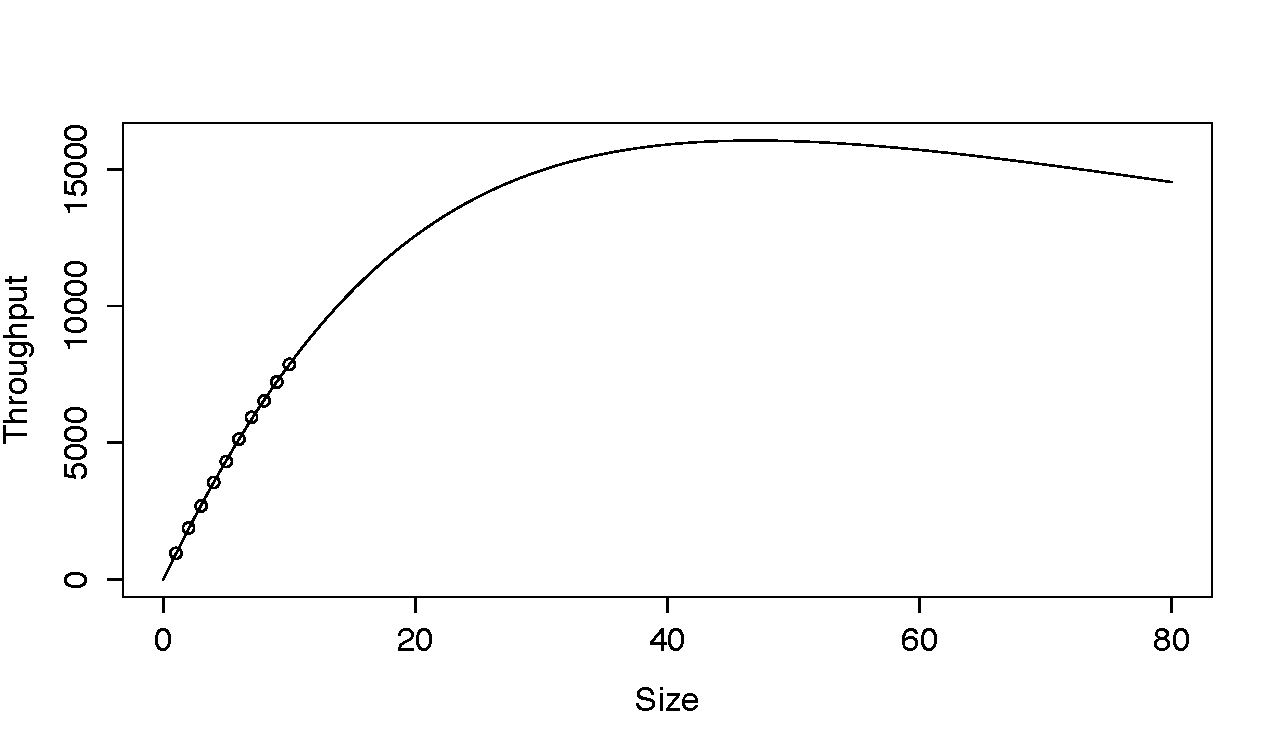
\includegraphics[width=.85\linewidth]{scalability/cisco-2}
\end{center}

Using the formula $N_{max}=\sqrt{(1-\sigma)/\kappa}$ from Equation \ref{n_max}, the USL predicts a
max of 16,049 queries per second at a concurrency of 46 threads.

I have a rule of thumb for using the USL to project out into the unknown. I've
seen so many systems that appear to be scaling beautifully---fitting the
USL cleanly, just as this one does---and then they hit rough waters, that I don't trust
anything farther out than twice the measured throughput or twice the
measured size, whichever comes first.\footnote{You'll see later why I don't just
use throughput, when I explain superlinear scaling.} And that's if I'm not seeing
telltale signs of leveling off or retrograde throughput. If I see those signs, I
lower my expectations accordingly. I will also include other information such as
CPU utilization to guide my estimates, if I have it, but in the absence of more
data this is a good way to keep expectations capped.

Back to the model: I have measurements only to $N=10$, where observed throughput
is 7,867, so I'm going to compute the predicted throughput at $N=20$. The result
is a throughput forecast of 12,572. This is less than twice my maximum
observed throughput, so I'll allow it. In my experience, it's an optimistic but
not unrealistic guess that I won't get more than about 12,500 queries per second
from this server. (As you may remember, this system topped out at 12,211 QPS.)

The outcome is that my system appears to be operating at about half of its
maximum capacity. However, as discussed previously, maximum throughput isn't
maximum {\itshape usable} capacity. Again, when the system is at its maximum
throughput, response time is probably terrible, and will be extremely
inconsistent. That's why it's more important to focus on the system's maximum
throughput within the constraints of a service level objective.

As a first step towards this, I can use average latency to help understand the
potential QoS end-users will get from this server. Again using the rearranged
form of the USL to forecast response times, I obtain the following:
\begin{center}
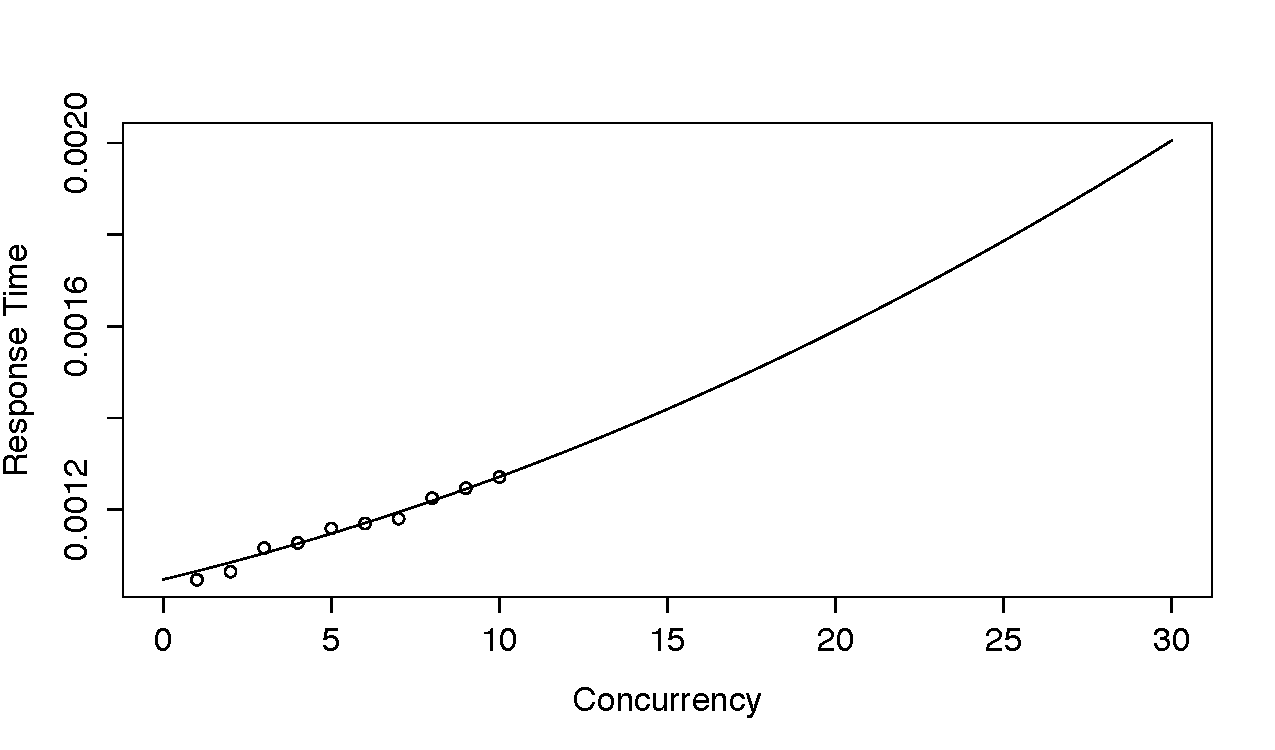
\includegraphics[width=.85\linewidth]{scalability/cisco-3}
\end{center}

Using the estimated coefficients and the formula for response time from Equation
\ref{r_n}, I can predict a mean response time
of 0.00159 seconds at 20 threads. Let's imagine that this is unacceptable; I
need mean response times to be 15ms or less. Solving the response time equation
as a function of latency lets me use it to compute the maximum usable
concurrency. The resulting equation has two roots; I'm only interested in the
positive one:
\begin{equation}
N(R)=\frac{\kappa-\sigma+\sqrt{\sigma^2+\kappa^2+2\kappa(2\lambda R+\sigma-2)}} {2\kappa}
\label{n_r}
\end{equation}

Plugging in an $R$ target of 0.0015 yields $N$ = 17, so if I want to avoid
violating my SLO I can't drive my server higher than approximately 11,450 QPS.
All of which is to say I'm actually at about two-thirds of my usable capacity; I
can grow traffic about 150\% before I get into trouble, if I'm lucky.

This process is something like what I might use if I were encountering this
server in the wild. It's not perfect; as Niels Bohr said, ``It's hard to make
predictions, especially about the future.'' Despite the uncertainty that
remains, this approach is much better than staring at a chart and thinking, ``I
don't know, it looks like it's scaling linearly and CPU utilization is only
10\%, so I guess we have a lot of headroom?'' You usually have less headroom
thank you think, because of how nonlinearly throughput and latency degrade.

The USL has a few nice properties that make it suitable for this type of
capacity planning:

\begin{itemize}
\item It's a ``black box'' technique, which uses data that's usually easy to get.
\item Gathering data and using regression to analyze it is also easy.
\item The USL is a relatively simple model, so people like me can understand the math. 
\item The USL is highly intuitive in comparison to most other approaches.
\end{itemize}

I would just repeat my caution that a lot of systems perform worse than the USL
predicts they will, because their degradation in scalability at larger sizes is
more severe than predicted. This is why I suggest viewing the USL's prediction
as optimistic: ``I won't count on being able to scale this system as high as the
USL predicts I can.''

You can also combine the USL with selected techniques from queueing theory, such
as the Square Root Staffing Rule, to forecast how much capacity is needed and
what quality of service it will provide. See the aforementioned
\href{https://www.vividcortex.com/resources/queueing-theory/}{queueing theory
book} for more on this topic.

\section{Using the USL to Improve Scalability}

One of the best uses of the USL is to explain {\itshape why} a system doesn't
scale as well as it might. Armed with this knowledge, you can get clues about
where to look for bottlenecks, so you might be able to alleviate them and
improve the system's scalability.  With practice, you'll also develop a mindset
of scalability, building intuition about which design decisions can cause
serious sublinearity.

An example will help illustrate. A few years ago PayPal published
\href{https://www.paypal-engineering.com/2013/11/22/node-js-at-paypal/}{benchmark
results} of a Java application they rewrote in NodeJS. I analyzed their
benchmark results and
\href{https://www.vividcortex.com/blog/2013/12/09/analysis-of-paypals-node-vs-java-benchmarks/}{wrote} about it on the VividCortex blog.
Here are the plots and the key scalability parameters:
\begin{center}
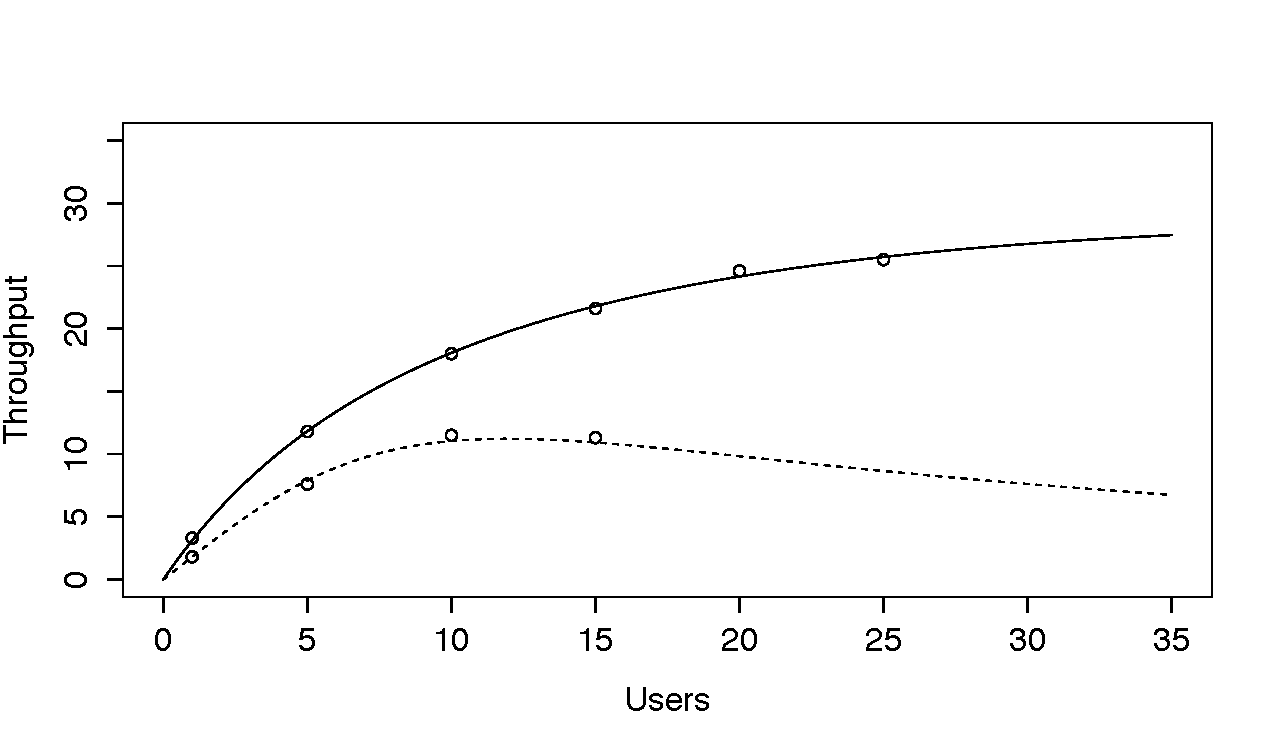
\includegraphics[width=.85\linewidth]{scalability/paypal}
\end{center}
\[
\begin{array}{lcc}
& \sigma & \kappa \\
\mbox{Java} & 0.000011 & 0.006323 \\
\mbox{NodeJS} &  0.080319 & 0.000222 \\
\end{array}
\]

These systems scale very differently,\footnote{Both of them scale pretty poorly,
in fact.} and for very different reasons.  In a nutshell, the Java benchmark
shows much higher crosstalk penalty, whereas the NodeJS benchmark exhibits more
contention from queueing and serialization. Examining the architectures of the
two systems reveals why: the Java app is multi-threaded and NodeJS is
single-threaded with an event loop, and the PayPal blog post even mentions that
they used ``a single core for the NodeJS application compared to five cores in
Java.''

This is a great real-life example of key scalability tenets:

\begin{itemize}
\item Avoid serialization and queueing; make things as parallel as possible.
\item Avoid crosstalk and synchronization.
\end{itemize}

If you're using the USL to model and analyze system scalability, another
valuable practice is to approach the USL as a pessimistic scenario. Synchronous
repairman queueing, the basis of the USL, is actually a worst-case in terms of
the amount of queueing delay that occurs in a system. This is another way of
saying that well-built systems theoretically ought to scale {\itshape at least}
as well as the USL predicts. This should prompt you to ask the question, ``why
is this system degrading more than it should?'' The answer is to look at
whether the system degrades because of contention (queueing, serialization) or
crosstalk (synchronization, communication, pairwise data interchange). If you
can identify the likely cause, you might suspect that you need to look at mutex
contention, for example.

One of the biggest changes in my mindset since learning to use the USL is that
it's possible, and important, to explain why systems behave as they do. As Neil
Gunther \href{https://twitter.com/DrQz/status/659086348729499649}{tweeted}, it's
no longer enough just to benchmark, measure, and present the results on a chart.
You can and should explain the results. As I
\href{https://twitter.com/xaprb/status/657354190109458433}{tweeted} myself,
``Benchmarking is good, publishing results is better, explaining results is
best. Publishing charts only (pictures without numbers) is sad.''

\newpage
\section{Thinking Critically About The USL}

For many people, the USL is a huge shift in mindset. I know it was for me. But
is it the be-all and end-all? Of course not.

Not only is the USL not the answer for every problem related to scalability
or capacity planning, sometimes it's hard to apply for the problems it
{\itshape can} solve. The examples I've shown thus far are remarkable in that
they're extremely clean data. Real-world systems often have noisy data that
doesn't ``look like'' the USL much at all. It may look more like something your
cat threw up on the screen. Even when there is a nice-looking shape to the data,
regression can produce unphysical results, or refuse to produce results.

And then there are the systems for which you have nice clean-room measurements,
highly reproducible, but they just don't seem to fit the USL very well. I could show
many examples. I've seen systems that appear to scale nicely, following the USL,
but suddenly flatline instead of continuing a graceful curve, or abruptly
degrade way faster than predicted---or the reverse, appearing to degrade more
{\itshape slowly} than predicted once you exit Amdahl territory and enter the
region where the higher-order terms prevail.  Here's an example:
\begin{center}
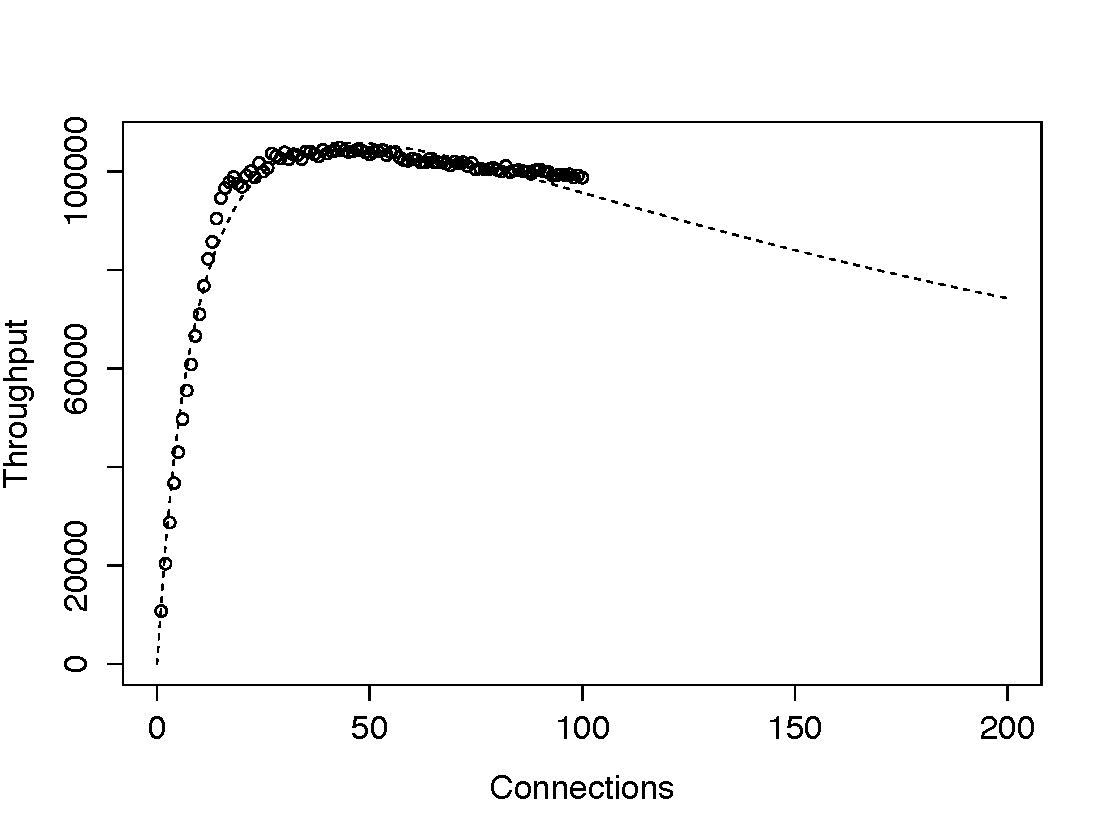
\includegraphics[width=.85\linewidth]{scalability/handlersocket}
\end{center}

Maybe this is queue saturation or resource saturation, or maybe it's something
else, but it is not something the USL has the capability to model or predict. If
you'd tried to predict this behavior by fitting the USL to the first dozen or so
data points, you'd get something like this:
\begin{center}
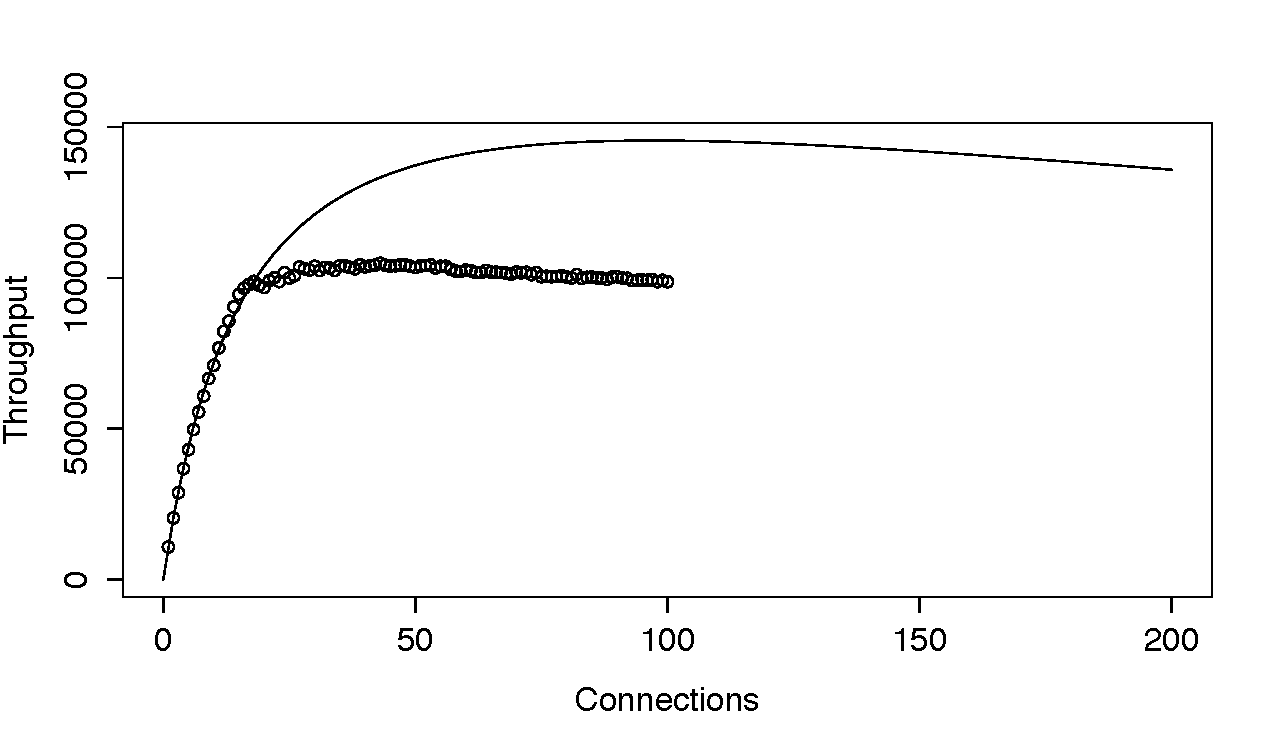
\includegraphics[width=.85\linewidth]{scalability/handlersocket-2}
\end{center}

The USL doesn't give you the tools to see those kinds of behavioral shifts
coming. There's no way to tell it how many servers are servicing queues, for
example. I've seen many benchmarks that fit the USL nicely with increasing
numbers of threads until there is one thread per physical CPU core; then there's
an abrupt change such as those in the diagram. I've seen others where a resource
such as network bandwidth becomes a limiting factor.

If the USL is incomplete, what is it good for? The answer is lots.

First of all, a model is better than no model. In the absence of a model
explaining the workings of system scalability, there isn't even a point of
comparison to assess your expectations and results. There's no frame of
reference to say, ``I think this system should scale better than it does,'' or
``This system's behavior makes no sense.'' Whether the USL is applicable to a
given problem or not, it still provides a framework. Without it, why not just
draw lines at will? You could get a set of French curves and follow your muse.
No one could say you're wrong.
\begin{center}

\includegraphics[width=.85\linewidth,trim={0 8cm 0 0},clip]{scalability/french_curve}
\end{center}

In an objective sense, the USL is both incomplete and wrong.  If it were
complete and correct, for example including knowledge about capped resources
such as number of CPUs (which is a vitally important parameter for queueing
theory problems) or network bandwidth, it would certainly describe more systems
and scenarios than it does in my experience. As Richard Feynman said in a 1964
lecture at Cornell University, ``If it disagrees with experiment, it’s wrong.
That simple statement is the key to science.''

This is not to say the USL isn't useful. As George E. P. Box famously said,
``all models are wrong, but some are useful.'' The USL is incredibly useful. But
we must not put it onto a pedestal and worship it.  

I'd also like to note that one could easily conjecture and analyze other
USL-like models. For example, many computer algorithms, such as those
that might perform pairwise interchange to cause the coherency penalty, can be shown
by analysis to be $\mathcal{O}(n\log{}n)$ instead of $\mathcal{O}(n^2)$. Perhaps
I could imagine that the quadratic $\kappa$ term doesn't really behave like its
worst-case, and the term could be replaced by a logarithmic term, like so?
\begin{equation}
X(N) = \frac{\lambda N}{1 + \sigma(N-1) + \kappa \log(N)(N-1)}
\label{usl_log}
\end{equation}

To give some visual intuition of how this differs from the accepted form of the
USL, here they are together on a single plot. The standard USL is the solid line
and the logarithmic variant is the dashed line.
\begin{center}
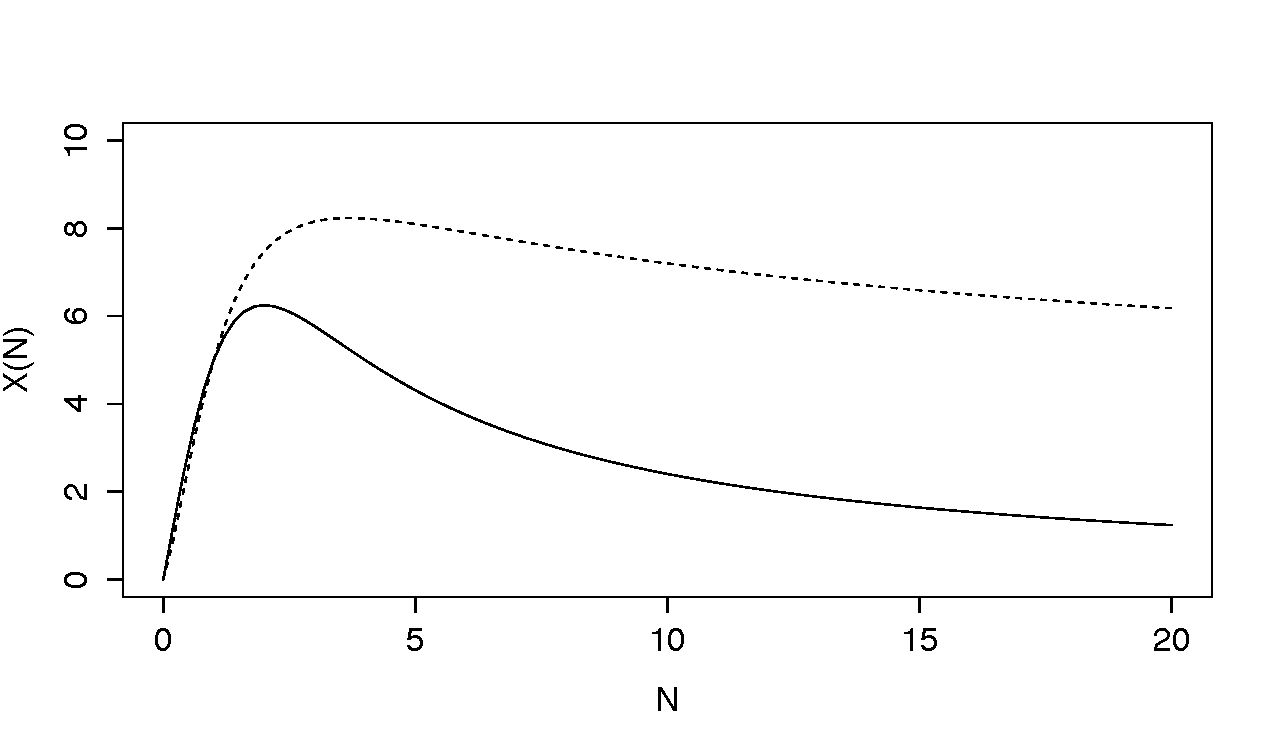
\includegraphics[width=.85\linewidth]{scalability/logscale}
\end{center}

You might think that you could choose parameters to the standard USL to make it
follow the dashed line better, but it doesn't work. The functions are of
different order and type, and won't behave the same.

Would this be a better model for the data I showed previously? Visually, it does
appear to model the observed data somewhat more closely:
\begin{center}
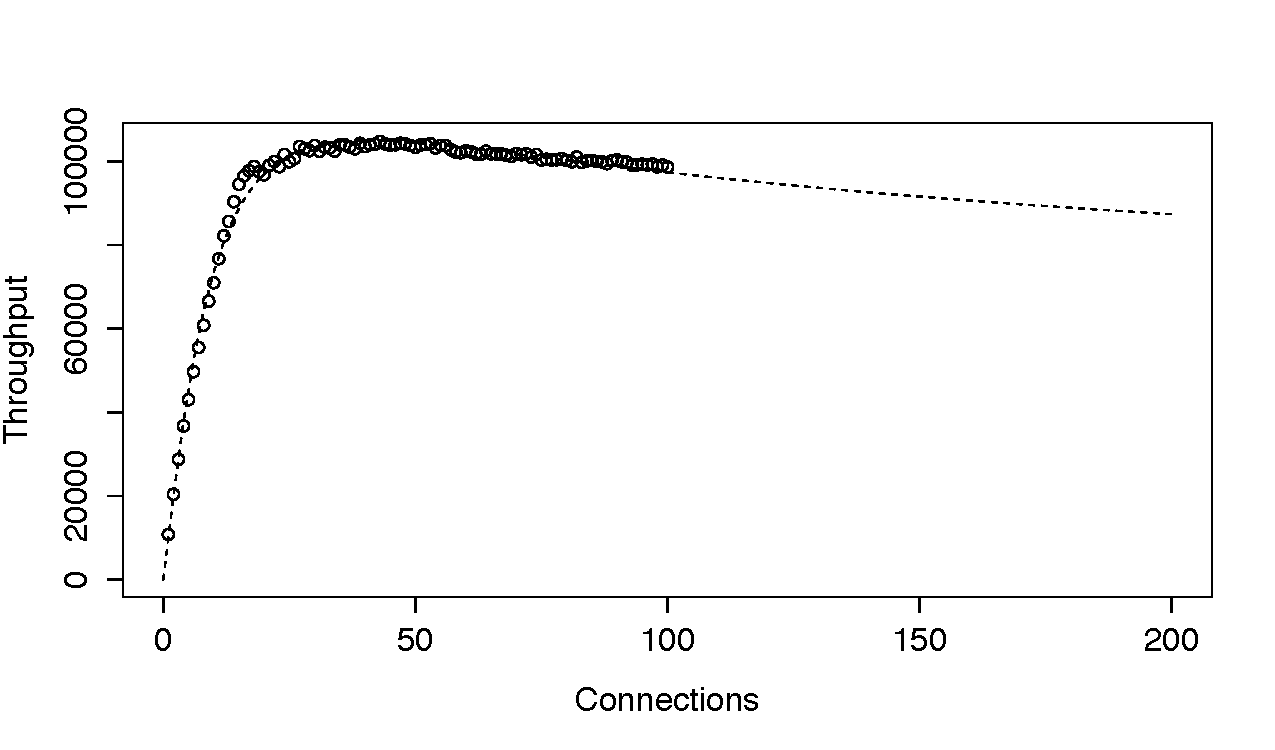
\includegraphics[width=.85\linewidth]{scalability/logscale-2}
\end{center}

Dr. Jayanta Choudhury has suggested changes to the USL to model cases such as this,
where resources apparently become saturated.  His 
Asymptotically Improved Super-Serial Law\footnote{See {\itshape Parameter
Estimation of Asymptotically Improved Super-serial Scalability Law} by Dr.
Jayanta Choudhury, of TeamQuest Corporation.} is slightly more complex:
\begin{equation}
X(N) = \frac{\lambda N}{1 + \sigma(N-1) + \sigma \kappa N^\beta (N-1)}
\label{aissl}
\end{equation}

The $\beta$ parameter ranges from 0 to 1, inclusive. The following plot shows
the logarithmic variant I proposed in a solid line, and the AISSL in a dashed
line. As you can see, the logarithmic variation fits the data better.
\begin{center}
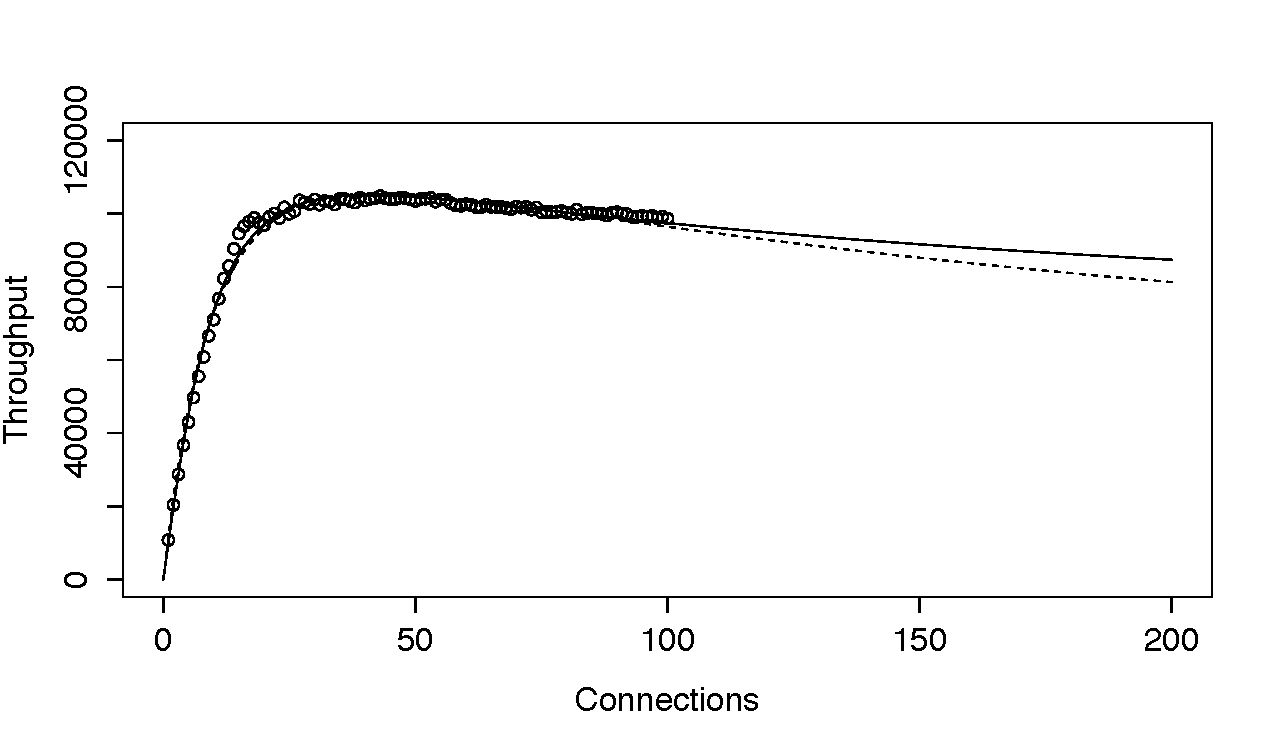
\includegraphics[width=.85\linewidth]{scalability/aissl}
\end{center}

Unfortunately it's a bit difficult to estimate parameters for the AISSL, making
it harder to use than the USL. 

As I'm sure you can imagine, you could play games like this all day long.
Dreaming up an idea is much easier than proving that it's correct or showing
how it might arise analytically from the underlying mechanisms as we understand
them to operate in the system.

The more practical way to look at the examples I've given in this section is to
stop trying to predict what happens after retrograde scalability or resource
saturation kicks in. There are at least two good reasons for taking this
pragmatic approach.

\begin{enumerate}
\item {\bfseries It's a different model.} The system's behavior is being
influenced by factors that weren't present at a smaller size. It's not just
different parameters, the entire model has changed, and it's doubtful that a
single model exists that could explain those wildly different behaviors.
\item {\bfseries It's pointless.}  When you see retrograde scaling, you know the
system has gone past the point where it's in trouble. Nothing good can come of
pushing it further, so why should you try to model how bad it is? It's a lost
cause with no practical purpose.
\end{enumerate}

\section{Superlinear Scaling}

I've spent some time analyzing the possible causes of sublinear scaling. Is
superlinear scaling possible? As I've worked with the USL over the years, I've
found a number of cases where systems apparently do scale superlinearly. It
manifests as a negative $\sigma$ coefficient and a USL curve that has a more
complex shape, rising above linear and then below again:
\begin{center}
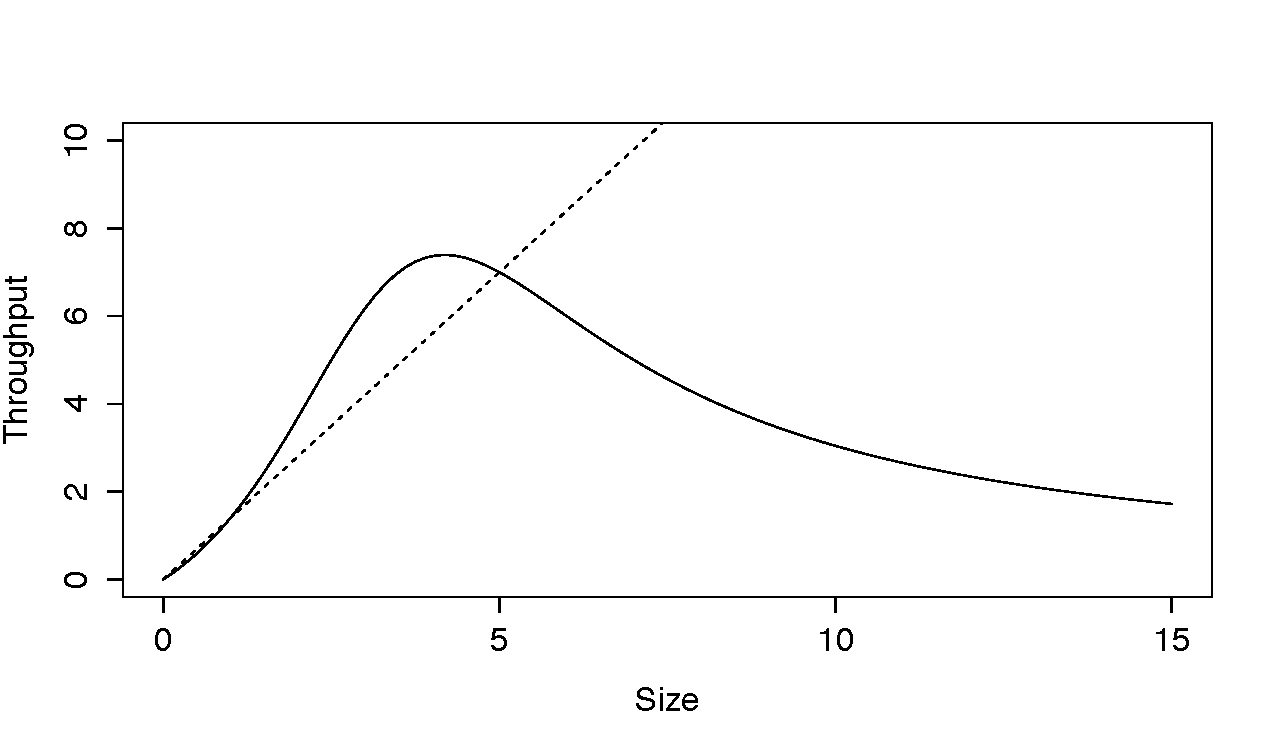
\includegraphics[width=.85\linewidth]{scalability/superlinear}
\end{center}

At first I dismissed this result as unphysical (how can there be less than zero
contention?), but after repeatedly seeing this happen and having many
conversations with Neil Gunther about it, I started to wonder. So did he, and
eventually he was able to reproduce and explain the effect on a
\href{https://queue.acm.org/detail.cfm?id=2789974}{large-scale Hadoop TeraSort
benchmark}.

The TeraSort case is quite a specific one. In the more general case, I would
explain superlinear scalability as a disproportionate scaling of some resource
relative to the load placed upon it, creating an economy of scale. For example,
adding more nodes to a clustered database system adds more memory; if the
dataset size is not scaled proportionately, then more of the data fits into
memory on each node, and access times improve relative to disk reads. Any
resource that is more efficient when shared than when used singly may cause this
effect.

It's worth noting that this initial boost, depending upon its cause, may be
countered by a correspondingly disproportionate ``payback'' later when
performance falls quickly below linearity again.

Another special case to be aware of is that some clustered systems behave
differently at sizes 1 and 2 than they do at 3 and above. For example, at size 1
there is no crosstalk or contention---it isn't a distributed system. At size 2
special-cases may be in play. At size 3 and above, usually generic algorithms
and techniques suited for any size $n$ are in use. Some clustered systems have
to be benchmarked or measured at larger sizes in order to avoid skew from these
effects.

Finally, negative $\sigma$ coefficients can arise from data that includes some
type of skew. For example, if you are measuring throughput at various levels of
concurrency and something is inflating the apparent concurrency measurements
(such as idling threads), all of your points will be shifted to the right on the
scatterplot. This can cause apparently superlinear scaling.

\newpage
\section{Other Scalability Models}

In addition to the USL and the variants I've already discussed, there are many
other potential models of scalability you could consider. In my opinion some are
good, some are useful, some are not. I also believe that there is much more work
to be done on this topic.

Some alternative theories, however, are just garbage. Chief amongst them is
``quadratic scalability.'' Observing that systems under increasing amounts of
load will first increase in throughput, then level off and begin to decline,
some people get the bright idea that they should ``fit a curve to it.'' The curve
is always a quadratic polynomial and the fitted curve ends up being a parabola
opening downwards. Let's see how this looks on the Cisco benchmark data 
once again:
\begin{center}
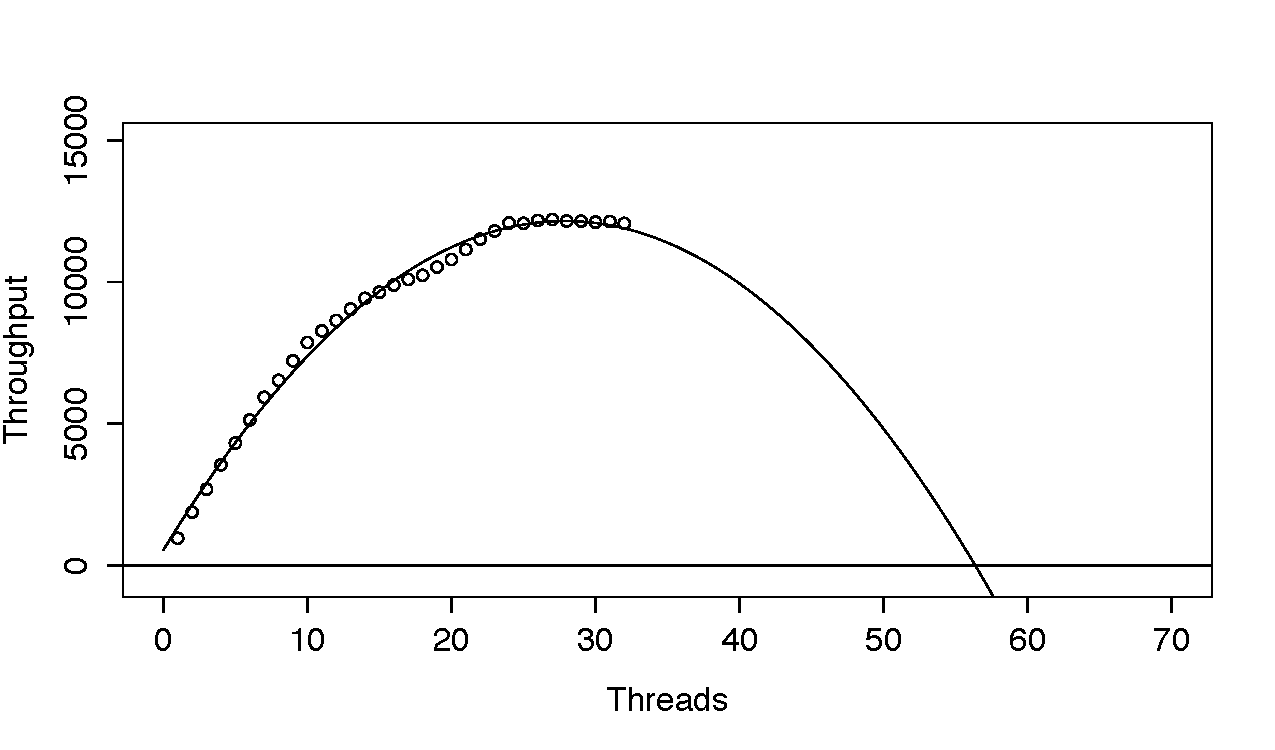
\includegraphics[width=.85\linewidth]{scalability/quadratic}
\end{center}

Look, Ma, it's a great fit! I don't even need to compute the $R^2$ value to know
that. There's just one problem: it predicts that at some point you'll achieve
negative throughput.

You should ignore this model because by definition it doesn't work. Rather than
use it, I'd suggest that you get out that French curve set again and get in
touch with your inner artist.

Another model that I've seen is latency as a function of throughput. Here
are three examples:

\begin{itemize}
\item New Relic's scalability chart, which plots latency as a function of
throughput and renders a smoothed line through the points. The line has no
predetermined form and doesn't express any particular model.
\item AppDynamics's scalability analysis feature does the same thing, but fits a
parabola through the lines instead of a polynomial of arbitrarily high degree.
\item Cockcroft headroom plots, by Adrian Cockcroft. These are also
latency-versus-throughput charts, but add some histograms and other useful
visual cues around the edges.
\end{itemize}

These three express essentially the same beliefs about the relationship between
variables--that throughput is an independent variable and determines latency.
AppDynamics models latency as quadratic, but otherwise
the differences among the three are relatively minor. Here's an example of a
\href{http://perfcap.blogspot.nl/2008/07/enhanced-headroom-plot-in-r.html}{Cockcroft
Headroom Plot}:
\begin{center}
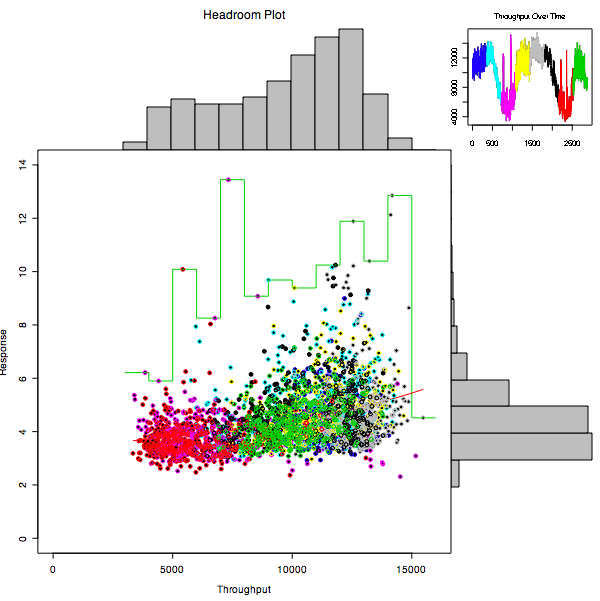
\includegraphics[width=.60\linewidth]{scalability/chpblog3}
\end{center}

As I have shown, the relationship between throughput and response
time is never quadratic under any circumstances, and is neither exponential 
nor a function of throughput unless $\kappa$ is zero.
In other words, you can't model the relationship in this way unless you
ignore the possibility of a nonzero $\kappa$, which I can attest is far from
rare. It is better to use a more capable model such as the USL.

\section{Hardware and Software Scalability}

I mentioned that Neil Gunther actually defines two forms of the USL, one for
hardware scaling and one for software. They're essentially the same equation,
with different Greek letters.

For most purposes it's not important to care about the distinction. However, it
is {\itshape very} important, in general, to have a firm grasp on the meaning of
the $X$ axis in the USL chart. I've been somewhat casual about it, essentially
treating it as a generic metric of size by which you scale the system or
workload, but now I will be more precise.

In fact there are at least three important dimensions of the work a system
performs, and how it scales, and these three interact with each other. A correct
understanding of the concepts is important to get sensible results:

\begin{enumerate}
\item {\bfseries Drivers.} The number of things producing work requests for the
system. In a benchmark, for example, this is typically the configured
concurrency of the benchmark---that is, the number of driver threads. It could
also be the number of connections to the database, the number of users on a web
application, and so on.
\item {\bfseries Servers.} The number of servers as defined in queueing theory. It could be the
number of CPUs in a server, the number of servers in a cluster, or the like.
\item {\bfseries Data.} The size of the dataset. This will most typically be in the usual
units---megabytes or gigabytes, number of rows---but will occasionally be the
number of logical partitions in the dataset (``shards''). A
\href{https://www.percona.com/blog/2011/02/28/is-voltdb-really-as-scalable-as-they-claim/}{VoltDB
benchmark} that I analyzed once needed to be couched in terms of partitions,
because of the configured per-partition redundancy.
\end{enumerate}

The key point in scalability analysis with the USL is that everything needs to be held
constant relative to the unit of scale you're using, so you are changing only
one variable at a time. If you're measuring scalability at different cluster
sizes, for example, you need to grow the number of driver threads and the data
size proportionately to the number of nodes in the cluster, so each node
receives the same amount and rate of work to perform upon the same amount of
data no matter the cluster size. (If you hold the dataset constant and increase
the number of nodes, you'll get superlinear scalability.)

% We've seen that the USL can be solved for a variety of dependent and independent
% variables, such as response time (latency). Yet another way to think about the
% USL is in terms of response time {\itshape reduction}, or speedup. I mentioned
% this briefly while motivating the introduction of Amdahl's Law, but a system
% that behaves like Amdahl's Law is probably less familiar to most readers.
% However, it's a perfect model to use for massively parallel processing (MPP)
% systems, which subdivide work and execute fractions of it in parallel, then
% combine the intermediate results into a final answer. In such a system, you can
% vary the degree of parallelism, measure how latency reduces, and produce a model
% of the system's scalability in terms of response time
% reduction.\footnote{Throughput and concurrency do not enter into the equation;
% you are not measuring aggregates of number of requests completed per time, but
% merely measuring the response time of individual requests at a concurrency of 1,
% by definition.}
% 
% To accomplish this, I need to make explicit what's been a bit bundled together
% into the USL when applied to hardware scalability. The assumption, not shown in
% Equation \ref{usl} directly, is that as you scale the number of servers $N$, you
% scale the drivers $D$ proportionately. In this way you hold the concurrency
% constant at each server. Again, I'm using the term ``server'' in the queueing
% theory sense of the word, e.g. nodes in the cluster, CPUs in the motherboard,
% degree of parallelism in the MapReduce job. Making this explicit in the USL
% looks like the following:
% \begin{equation}
% X = \frac{\lambda \frac{D}{N}}{1 + \sigma(\frac{D}{N} - 1) + \kappa
% \frac{D}{N}(\frac{D}{N}-1)}
% \label{usl_drivers}
% \end{equation}
% 
% Naturally, if the purpose is to measure speedup of individual requests, this
% becomes
% \begin{equation}
% X = \frac{\lambda \frac{1}{N}}{1 + \sigma(\frac{1}{N} - 1) + \kappa
% \frac{1}{N}(\frac{1}{N}-1)}
% \label{usl_speedup}
% \end{equation}

\section{Conclusions}

The Universal Scalability Law is a wonderfully versatile, easy-to-apply, yet
formal framework for modeling, thinking about, and analyzing scalability and
performance. It applies to many different situations, as long as you can define
the variables correctly. It even explains why human organizations (companies and
teams) struggle as they grow. As anyone who's managed a growing company knows,
the chief scaling problem in a big company is a communications problem.

In this book I've given you a whirlwind tour of modeling scalability and
performance with the USL. A few of the key takeaways are as follows:

\begin{itemize}
\item Scalability is a formal concept that is best defined as a mathematical
function.
\item Linear scalability means equal return on investment. Double down on
workers and you'll get twice as much work done; add twice as many nodes and
you'll increase the maximum capacity twofold. Linear scalability is oft claimed
but seldom delivered.
\item Systems scale sublinearly because of contention, which adds queueing
delay, and crosstalk, which inflates service times. The penalty for contention
grows linearly and the crosstalk penalty grows quadratically.
\item Contention causes throughput to asymptotically approach the
reciprocal of the serialized fraction of the workload. If your workload is 5\%
serialized you'll never grow the effective speedup by more than 20-fold.
\item Crosstalk causes the system to regress. The harder you try to push systems
with crosstalk, the more time they spend fighting amongst themselves.
\item To build scalable systems, avoid contention (serialization) and crosstalk
(synchronization).
The contention and crosstalk penalties degrade system scalability and
performance {\itshape much} faster than you'd think. Even tiny amounts of
serialization or pairwise data synchronization cause big losses in efficiency.
\item If you can't avoid crosstalk, partition (shard) into smaller systems that will
lose less efficiency by avoiding the explosion of service times at larger sizes.
\item To model systems with the USL, obtain measurements of throughput at
various levels of load or size, and use regression to estimate the parameters to
Equation \ref{usl}.
\item To forecast scalability beyond what's observable, be pessimistic and treat
the USL as a best-case scenario that won't really happen. Use Equation
\ref{n_max} to forecast the maximum possible throughput, but don't forecast too
far out. Use Equation \ref{r_n} to forecast response time.
\item Use your judgment to predict limitations that USL can't see, such as
saturation of network bandwidth or changes in the system's model when all of the
CPUs become busy.
\item Use the USL to explain why systems aren't scaling well. Too much queueing?
Too much crosstalk? Treat the USL as a pessimistic model and demand that your
systems scale at least as well as it does.
\item If you see superlinear scaling, check your measurements and how you've set
up the system under test. In most cases $\sigma$ should be positive, not
negative. Make sure you're not varying the system's dimensions relative to each
other and creating apparent superlinear efficiencies that don't really exist.
\item It's fun to fantasize about models that might match observed system
behavior more closely than the USL, but the USL arises analytically from how we
know queueing systems work. Invented models might not have any basis in reality.
Besides, the USL usually models systems extremely well up to the point of
inflection, and modeling what happens beyond that isn't as interesting as
knowing {\itshape why} it happens.
\item Never trust a scatterplot with an arbitrary curve fit through it unless
you know why that's the right curve. Don't confuse the USL, hockey stick charts
from queueing theory, or other charts that just happen to have similar shapes.
\end{itemize}

The USL succeeds because it encapsulates many different effects implicitly, and
doesn't require you to capture arcane measurements that may be impossible to
obtain. It's simpler to use and often gives better results than many other types of
forecasting tools, such as Erlang C formulas. For the same reasons, it's limited
in its predictive ability. But remember: as Neil Gunther says, ``Models don't
get confused, only modelers do.''

Many thanks to Dr. Neil Gunther, Cary Millsap, John Allspaw, Adrian Cockcroft,
John Miller, Dr.  Nathaniel Schwartz, Vadim Tkachenko, Peter Zaitsev, Dr.
Jayanta Choudhury, and others too numerous to mention. They deserve credit for
most of the things I've gotten right in this book. The errors, confusions, and
thickheadedness are all mine. I also beg Neil Gunther's perpetual forgiveness in
advance.

\section{Further Reading}

The Universal Scalability Law is only a couple of decades old and there is not a
great deal of literature about it. Interested readers should purchase the
canonical books from Dr. Neil J. Gunther. I include a variety of other excellent
reading in the list below, but Neil Gunther's books are the definitive sources.

\begin{itemize}
\item \href{http://www.springer.com/book/978-3-540-26138-4}{\itshape Guerrilla Capacity Planning} by Neil Gunther. This book is more or less the canonical text.
\item {\itshape Analyzing Computer System Performance With Perl::PDQ} by Neil
Gunther, which introduces the background to the USL.
\item {\itshape Practical Performance Analyst} by Neil Gunther.
\item {\itshape Forecasting MySQL Scalability with the Universal Scalability Law} by Baron Schwartz and Ewen Fortune.
\item {\itshape Fundamentals of Queueing Theory} by Gross and Harris.
\item {\itshape Practical Queueing Analysis} by Mike Tanner.
\item {\itshape Probability, Statistics, and Queueing Theory} by Allen.
\item {\itshape Capacity Planning for Web Performance} by Menasc\'e and Almeida.
\item {\itshape The Art of Computer Systems Performance Analysis} by Jain.
\end{itemize}

\newpage

\begin{about}	% Build "About VividCortex"
VividCortex is a SaaS database performance monitoring platform. The database is the heart of most applications, but it's also the part that's hardest to scale, manage, and optimize even as it's growing 50\% year over year. VividCortex has developed a suite of unique technologies that significantly eases this pain for the entire IT department. Unlike traditional monitoring, we measure
and analyze the system's work and resource consumption. This leads directly to better performance for IT as a whole, at reduced cost and effort.
\end{about}
\makeresources	% Build "Related Resources"
\end{document}
